\documentclass[../main.tex]{subfiles}
\graphicspath{{resources/}{resources/android_res}}
 
\begin{document}

\section{Androidos alkalmazás elkészítése}
    \subsection{Androidról általában}
        Android a világ legnépszerűbb mobil operációs rendszere. Több milliárd eszközön fut, mint például a telefonokon, órákon, táblagépeken, TV-ken, és még sok máson. 
        Különböző alakú és méretű eszközökön egyaránt elfut, ezzel óriási flexibilitást biztosítva az alkalmazás fejlesztők számára. 
        A nemrégiben megjelent \textit{Android Things} lehetővé teszi az okos, internetre csatlakoztatott eszközök építését, nem csak általános, hanem kereskedelmi és ipari felhasználásra is. A meglévő Androidos fejlesztői eszközökön kívül elérhetővé válik az alacsony szintű I/O könyvtárak kezelése is. 
        
        Azért döntöttem az Android alapú vezérlés mellett, mert megbízható, biztonságos, mindezek mellett nagyon olcsó eszközökön is tökéletesen működik. 
        
        \begin{figure}[h!]
            \centering
            
\includegraphics[width=7cm]{android_res/android_logo.png}
            \caption{Android logó}
            \label{fig:android_logo}
        \end{figure}
        
    \subsection{Android Platform felépítése} %https://developer.android.com/guide/platform/
        Az Android egy nyílt forráskódú, Linux alapú szoftvercsomag, amely számos eszköz és formai tényező számára készült. A ~\ref{fig:android_szoftvercsomag}. ábra mutatja a platform legfontosabb összetevőit.
        \begin{figure}[h!]
            \centering
            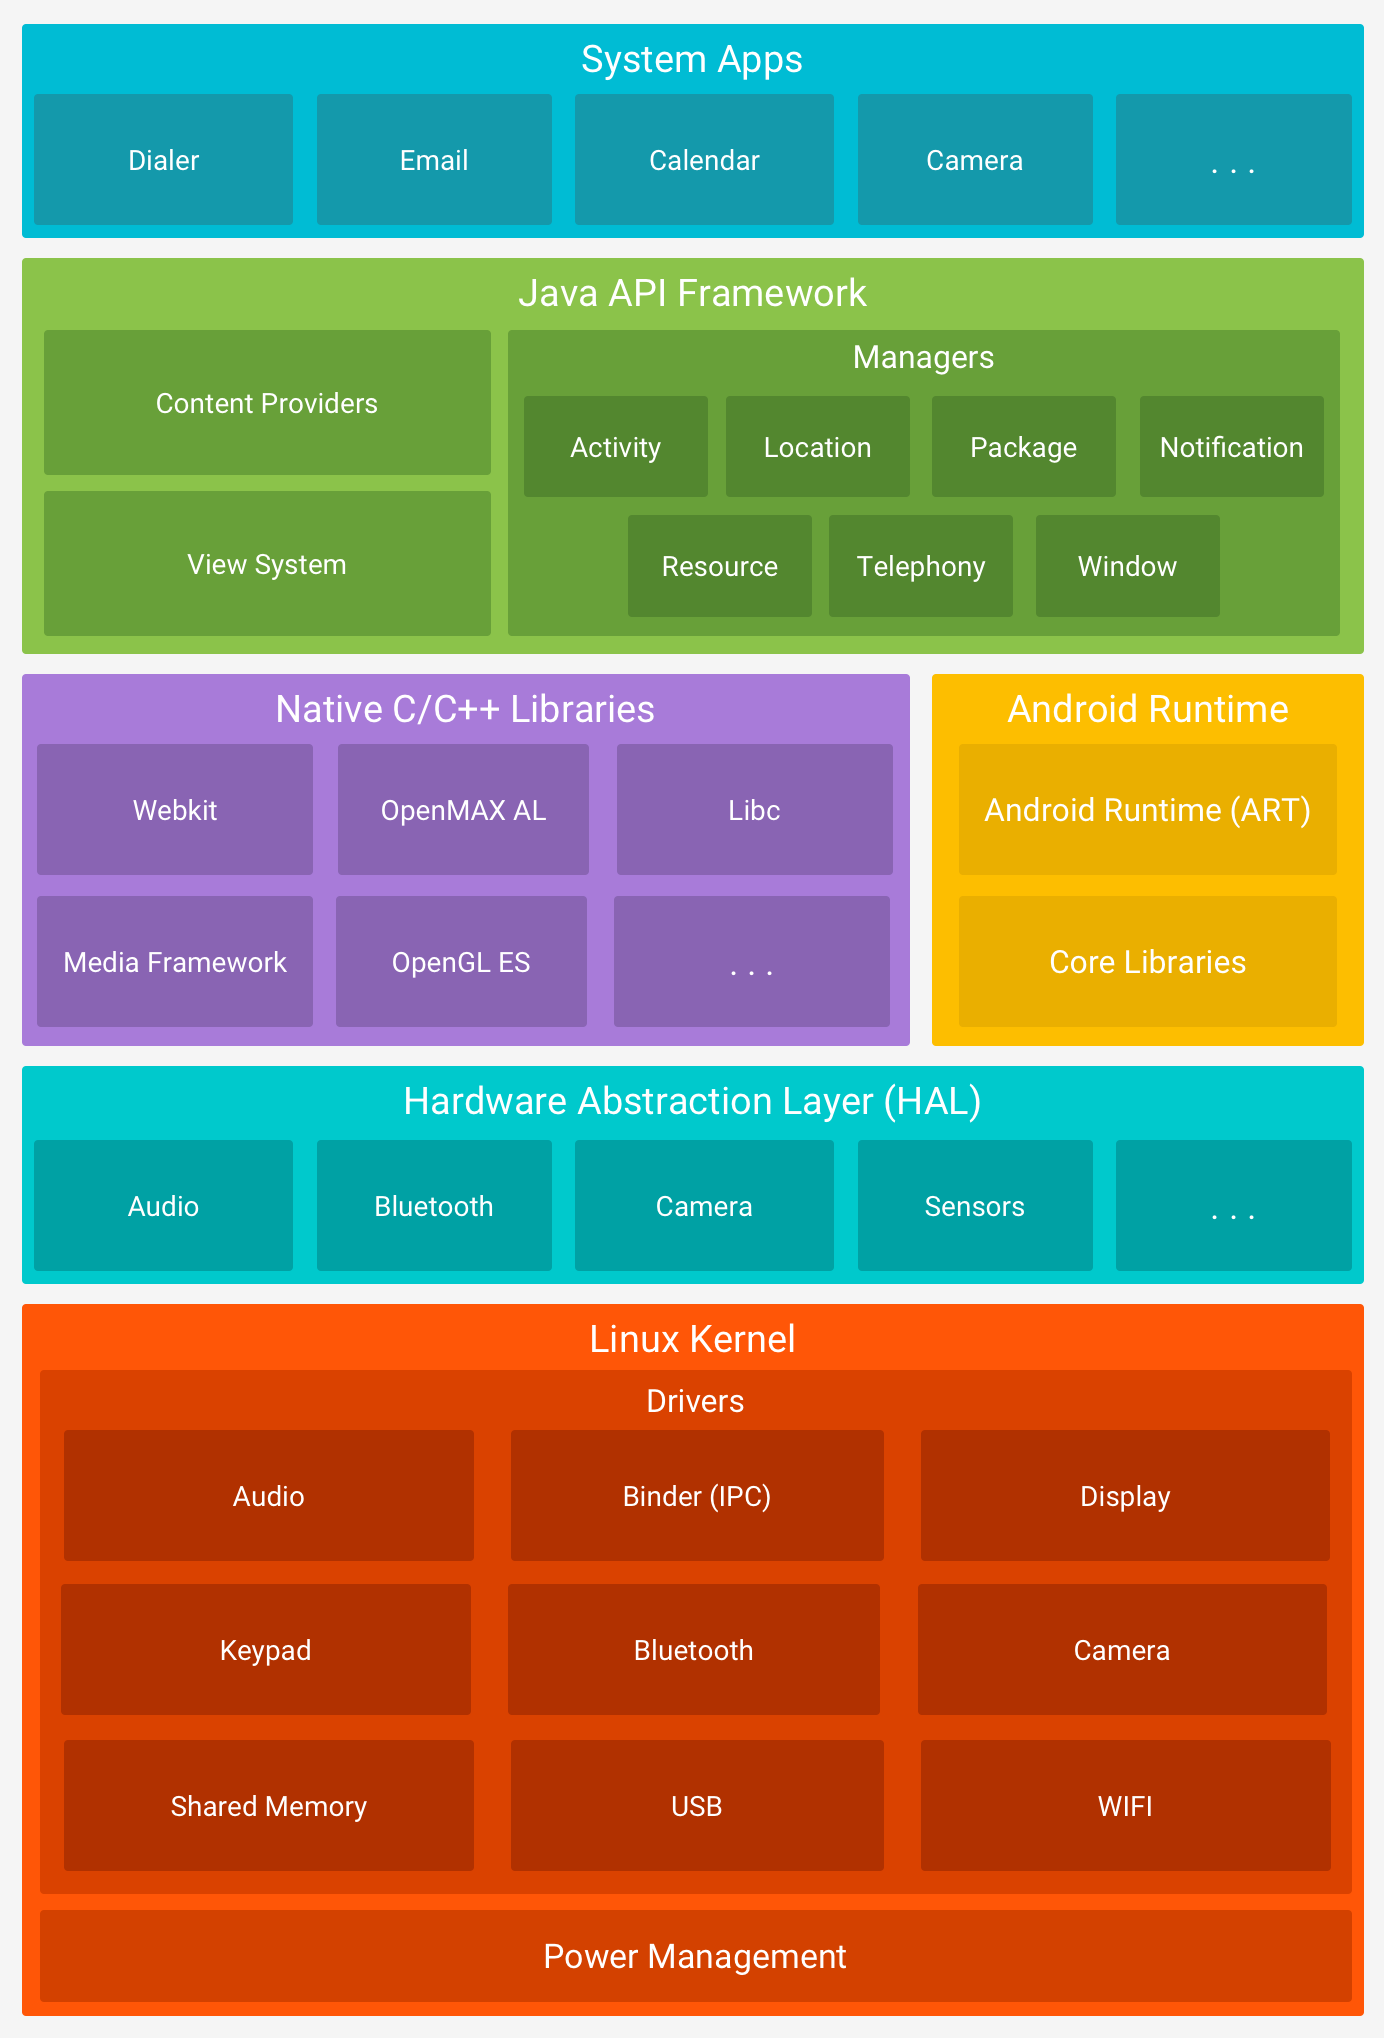
\includegraphics[width=11cm]{android_res/android_szoftvercsomag.png}
            \caption{Android szoftvercsomag}
            \label{fig:android_szoftvercsomag}
        \end{figure}
        
        \subsubsection{A Linux kernel}
            Az Android platform alapja a Linux kernel. Például az Android Runtime (ART) a Linux kernelen alapszik, ami magában rejti az olyan funkciókat, mint a szálkezelés és az alacsonyszintű  memóriakezelés.
            A Linux kernel segítségével az Android kihasználhatja a kulcsfontosságú biztonsági funkciókat, és lehetővé teszi az eszközgyártók számára, hogy egy jól ismert rendszermaghoz hardver-illesztőprogramokat fejlesszenek ki.
            
        \subsubsection{Hardware Abstacion Layer (HAL)}
             A hardver absztrakciós réteg (HAL) olyan szabványos felületet, amely a hardver képességeit a magasabb szintű Java API keretrendszer számára biztosítja. A HAL több könyvtármodulból áll,  amelyek mindegyike egy adott típusú hardverösszetevőhöz, például a kamerához vagy a bluetooth modulhoz ad hozzáférést. Amikor egy API hívás érkezik egy adott hardverhez, akkor az Android rendszer betölti a megfelelő komponenshez tartozó könyvtár-modulokat.
            
        \subsubsection{Android Runtime (ART)}
            Az Android 5.0-s verzióját (API-szint 21) vagy újabb verziót használó eszközök esetében minden alkalmazás saját folyamatában és az saját példányán fut. Az ART olyan virtuális gépek futtatására íródott, amelyek alacsony memóriájú eszközökön futtatnak DEX-fájlokat, speciálisan az Androidra tervezett bytecode formátumot, amely a minimális memóriahasználatra optimalizált. A toolchainek lefordítják a Java forrásokat DEX bytecode-ba, amelyek már futtathatóak az Android platformon.
            
        \subsubsection{Natív C/C++ könyvtárak}
            Számos fő Android rendszer komponens és szolgáltatás, mintpéldául az ART és a HAL, amelyek natív kódokon alapuló könyvtárokon alapszanak. Az Android platform a Java keretrendszernek megadja a hozzáférést ezekhez a könyvtárakhoz. Például hozzáférhetünk az OpenGL ES-hez az Android keretrendszer Java OpenGL API-val és így 2D-s és 3D-s grafikákat készíthetünk az alkalmazásainkban.
            
            Ha olyan alkalmazást fejlesztünk, amiben C/C++ kód van, akkor használhatjuk az Android NDK-t hogy a natív kódból közvetlenül hozzáférhessünk ezekhez a könyvtárakhoz.
            
        \subsubsection{Java API keretrendszer //TODO}
            
            
        \subsubsection{Rendszer alkalmazások //TODO}
            
        
    \subsection{Android alkalmazások felépítése //TODO} %https://developer.android.com/guide/components/fundamentals
        There are four different types of app components:

            Activities
            
            Services
            
            Broadcast receivers
            
            Content providers

        
    
        
        Felhasználói felület
        A felhasználói felület a manapság gyakori 5.5-inch-es, 16:9-es képarányú, FullHD (1920x1080) felbontású mobiltelefonokra terveztem és valósítottam meg, de ennél nagyobb kijelzőjű tableteken is elfut az alkalmazás.
        
        
    \subsection{Az elkészült alkalmazás funkciói és felhasználói kézikönyv}
        Az alkalmazás indításakor valamilyen WiFi hálózathoz csatlakozva vagyunk, akkor az
        alapértelmezett Simple Color Picker képernyő töltődik be, amit később a beállításokban módosíthatunk kedvünk szerint. Egyébként pedig egy hibát jelző oldal, amin a csatlakozás gombra kattintva eljuthatunk a készülékünk WiFi beállítások menüjébe, és ott csatlakozhatunk a hálózatra (Ábra: ~\ref{fig:wifi_err_01},~\ref{fig:wifi_err_02},~\ref{fig:wifi_err_03}).
        
        %\subsubsection{Hibaelhárítás}
             
            \begin{figure}[h!]
                \begin{floatrow}
                    \ffigbox{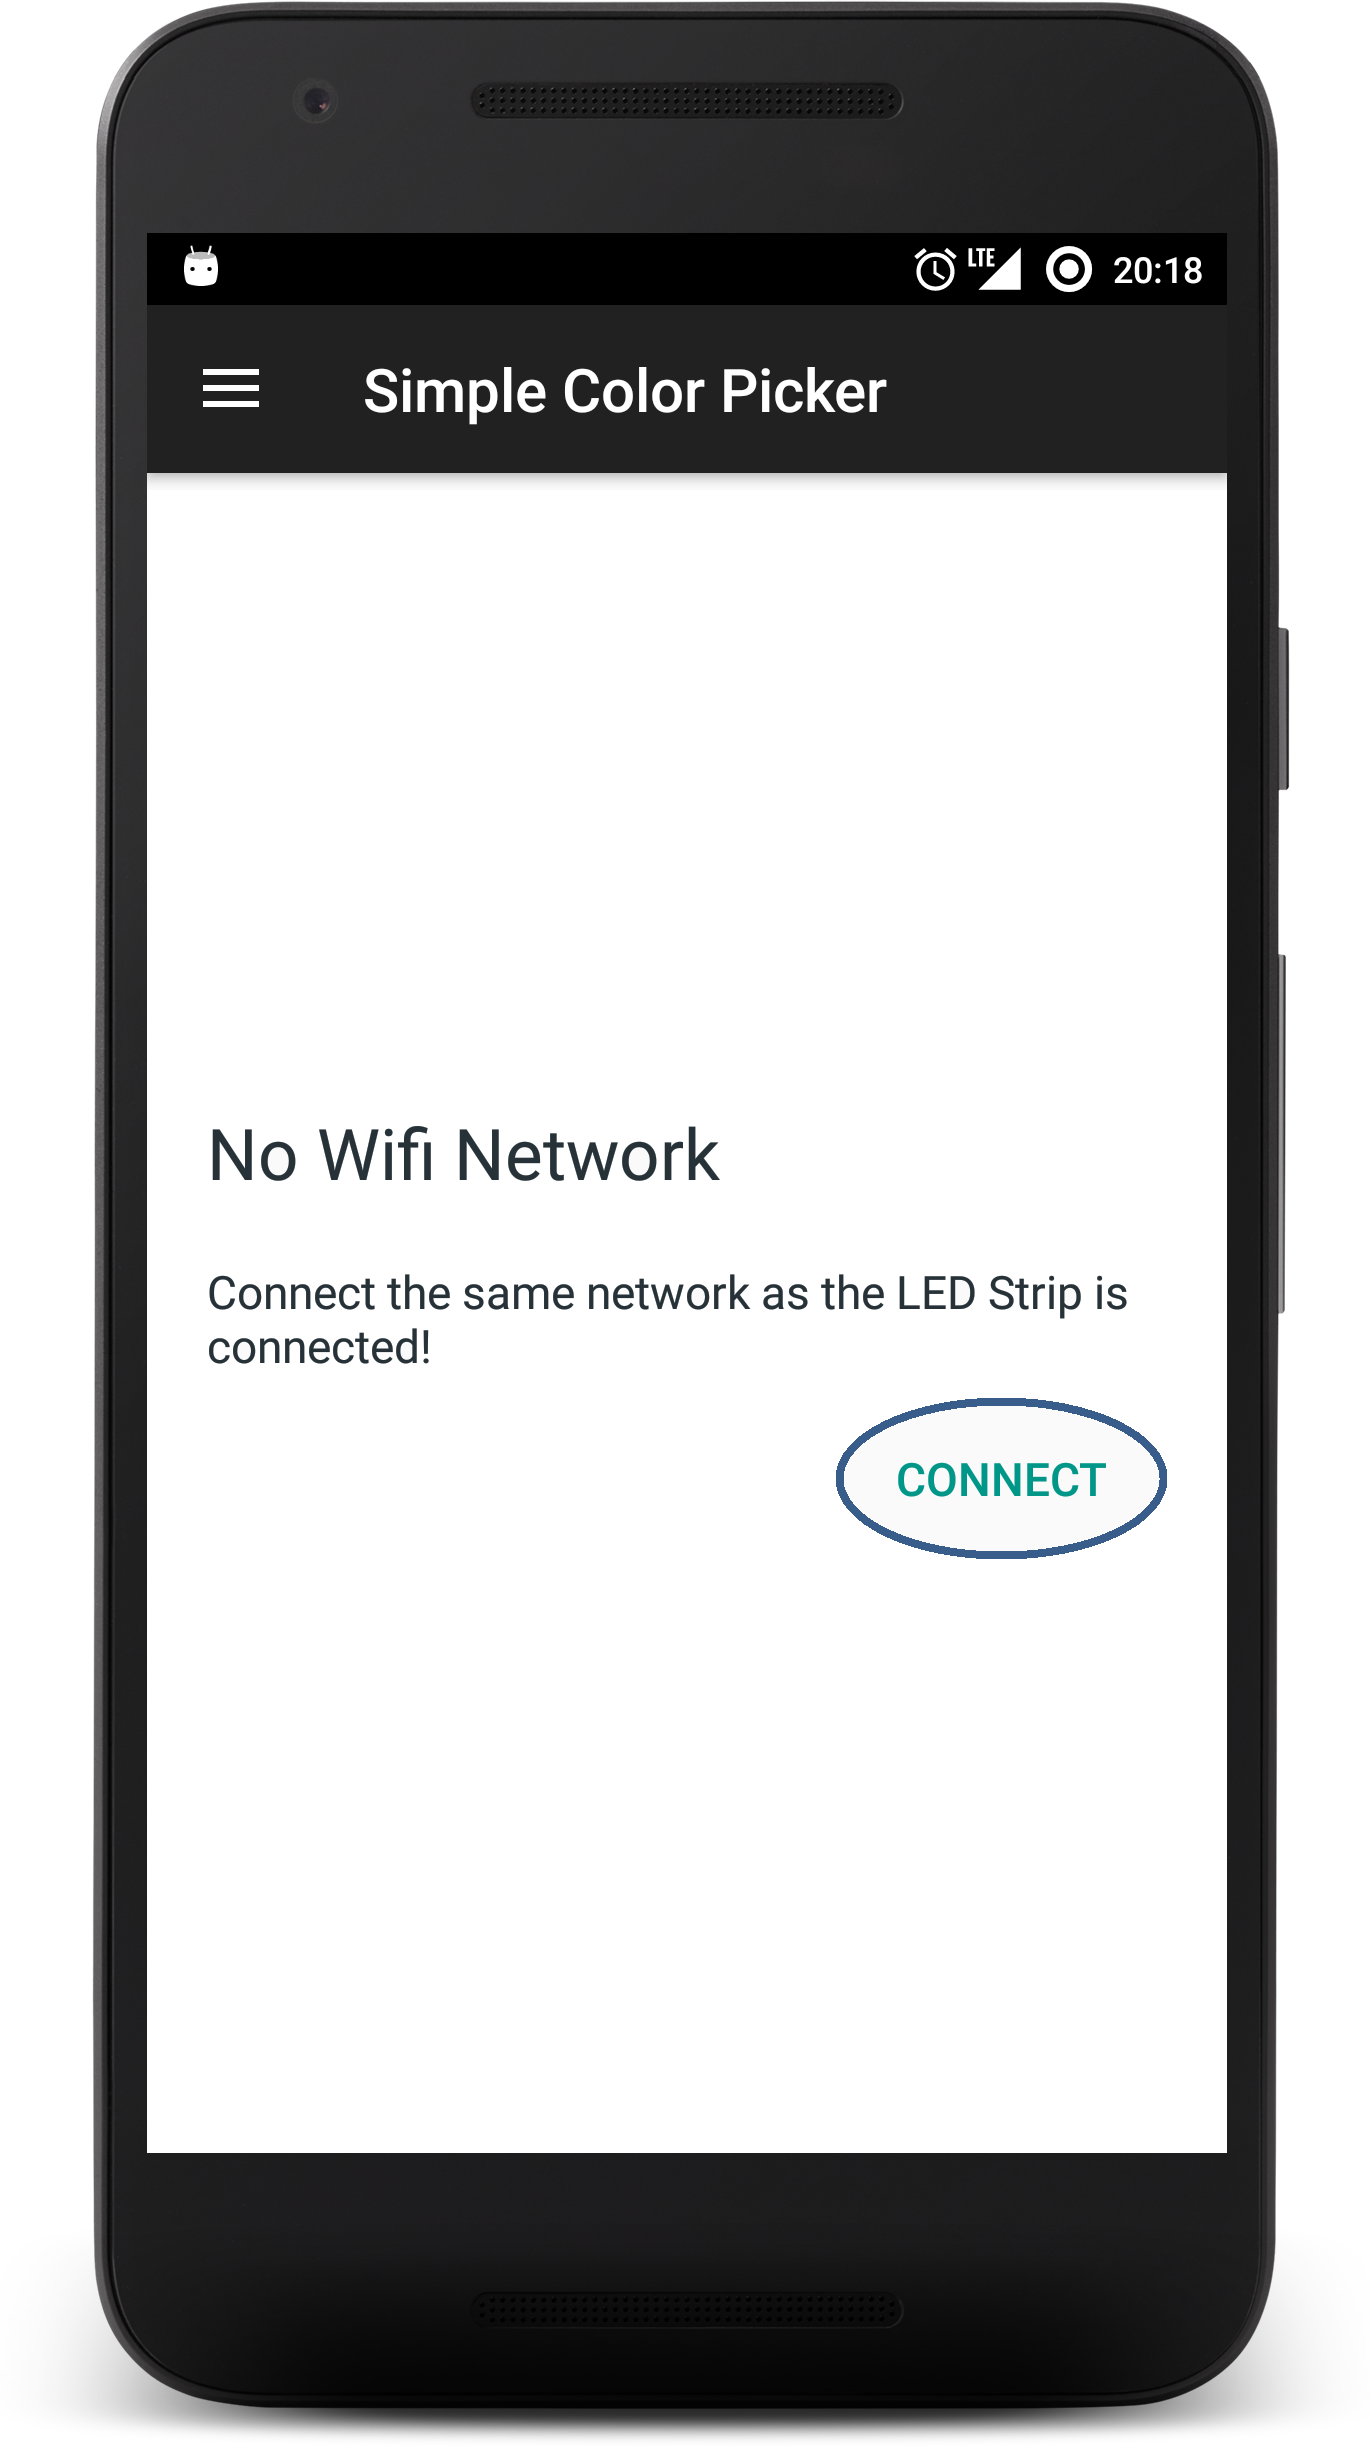
\includegraphics[width=5cm]{android_res/screen_pictures/wifi_err_01.png}}{\caption{Koppintson a csatlakozás gombra!}\label{fig:wifi_err_01}}
                    \ffigbox{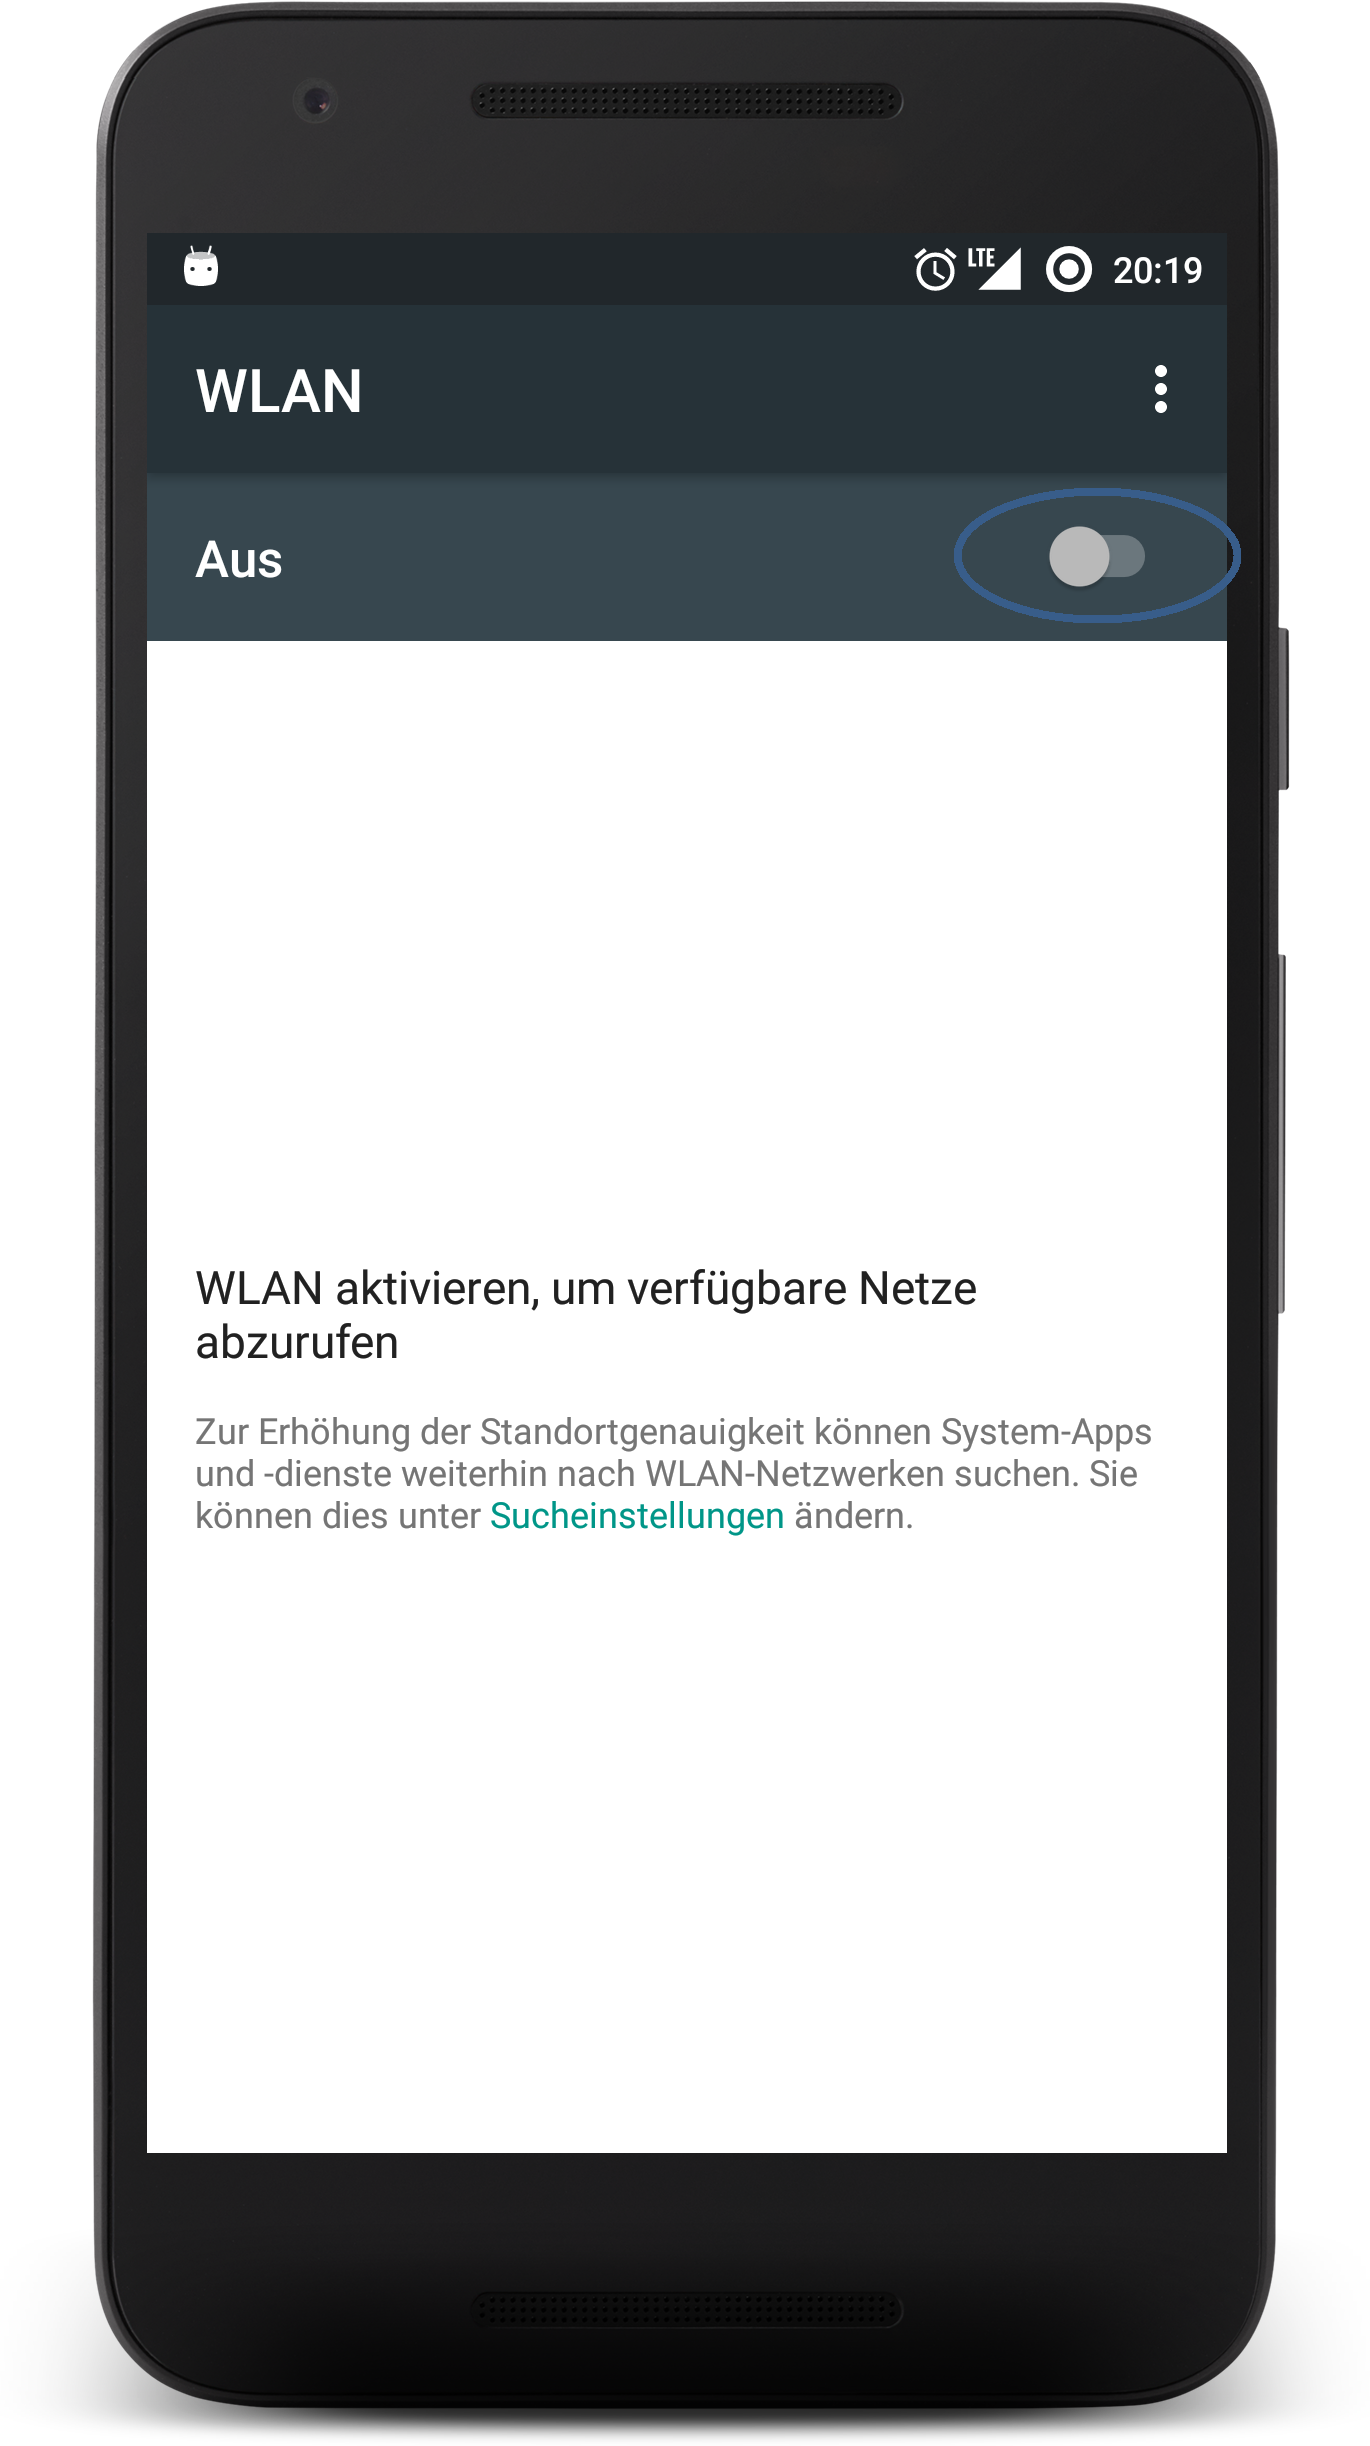
\includegraphics[width=5cm]{android_res/screen_pictures/wifi_err_02.png}}{\caption{Majd a bekapcsolásra!}\label{fig:wifi_err_02}}
                \end{floatrow}
            \end{figure}
            \begin{figure}[!h]
                \centering
                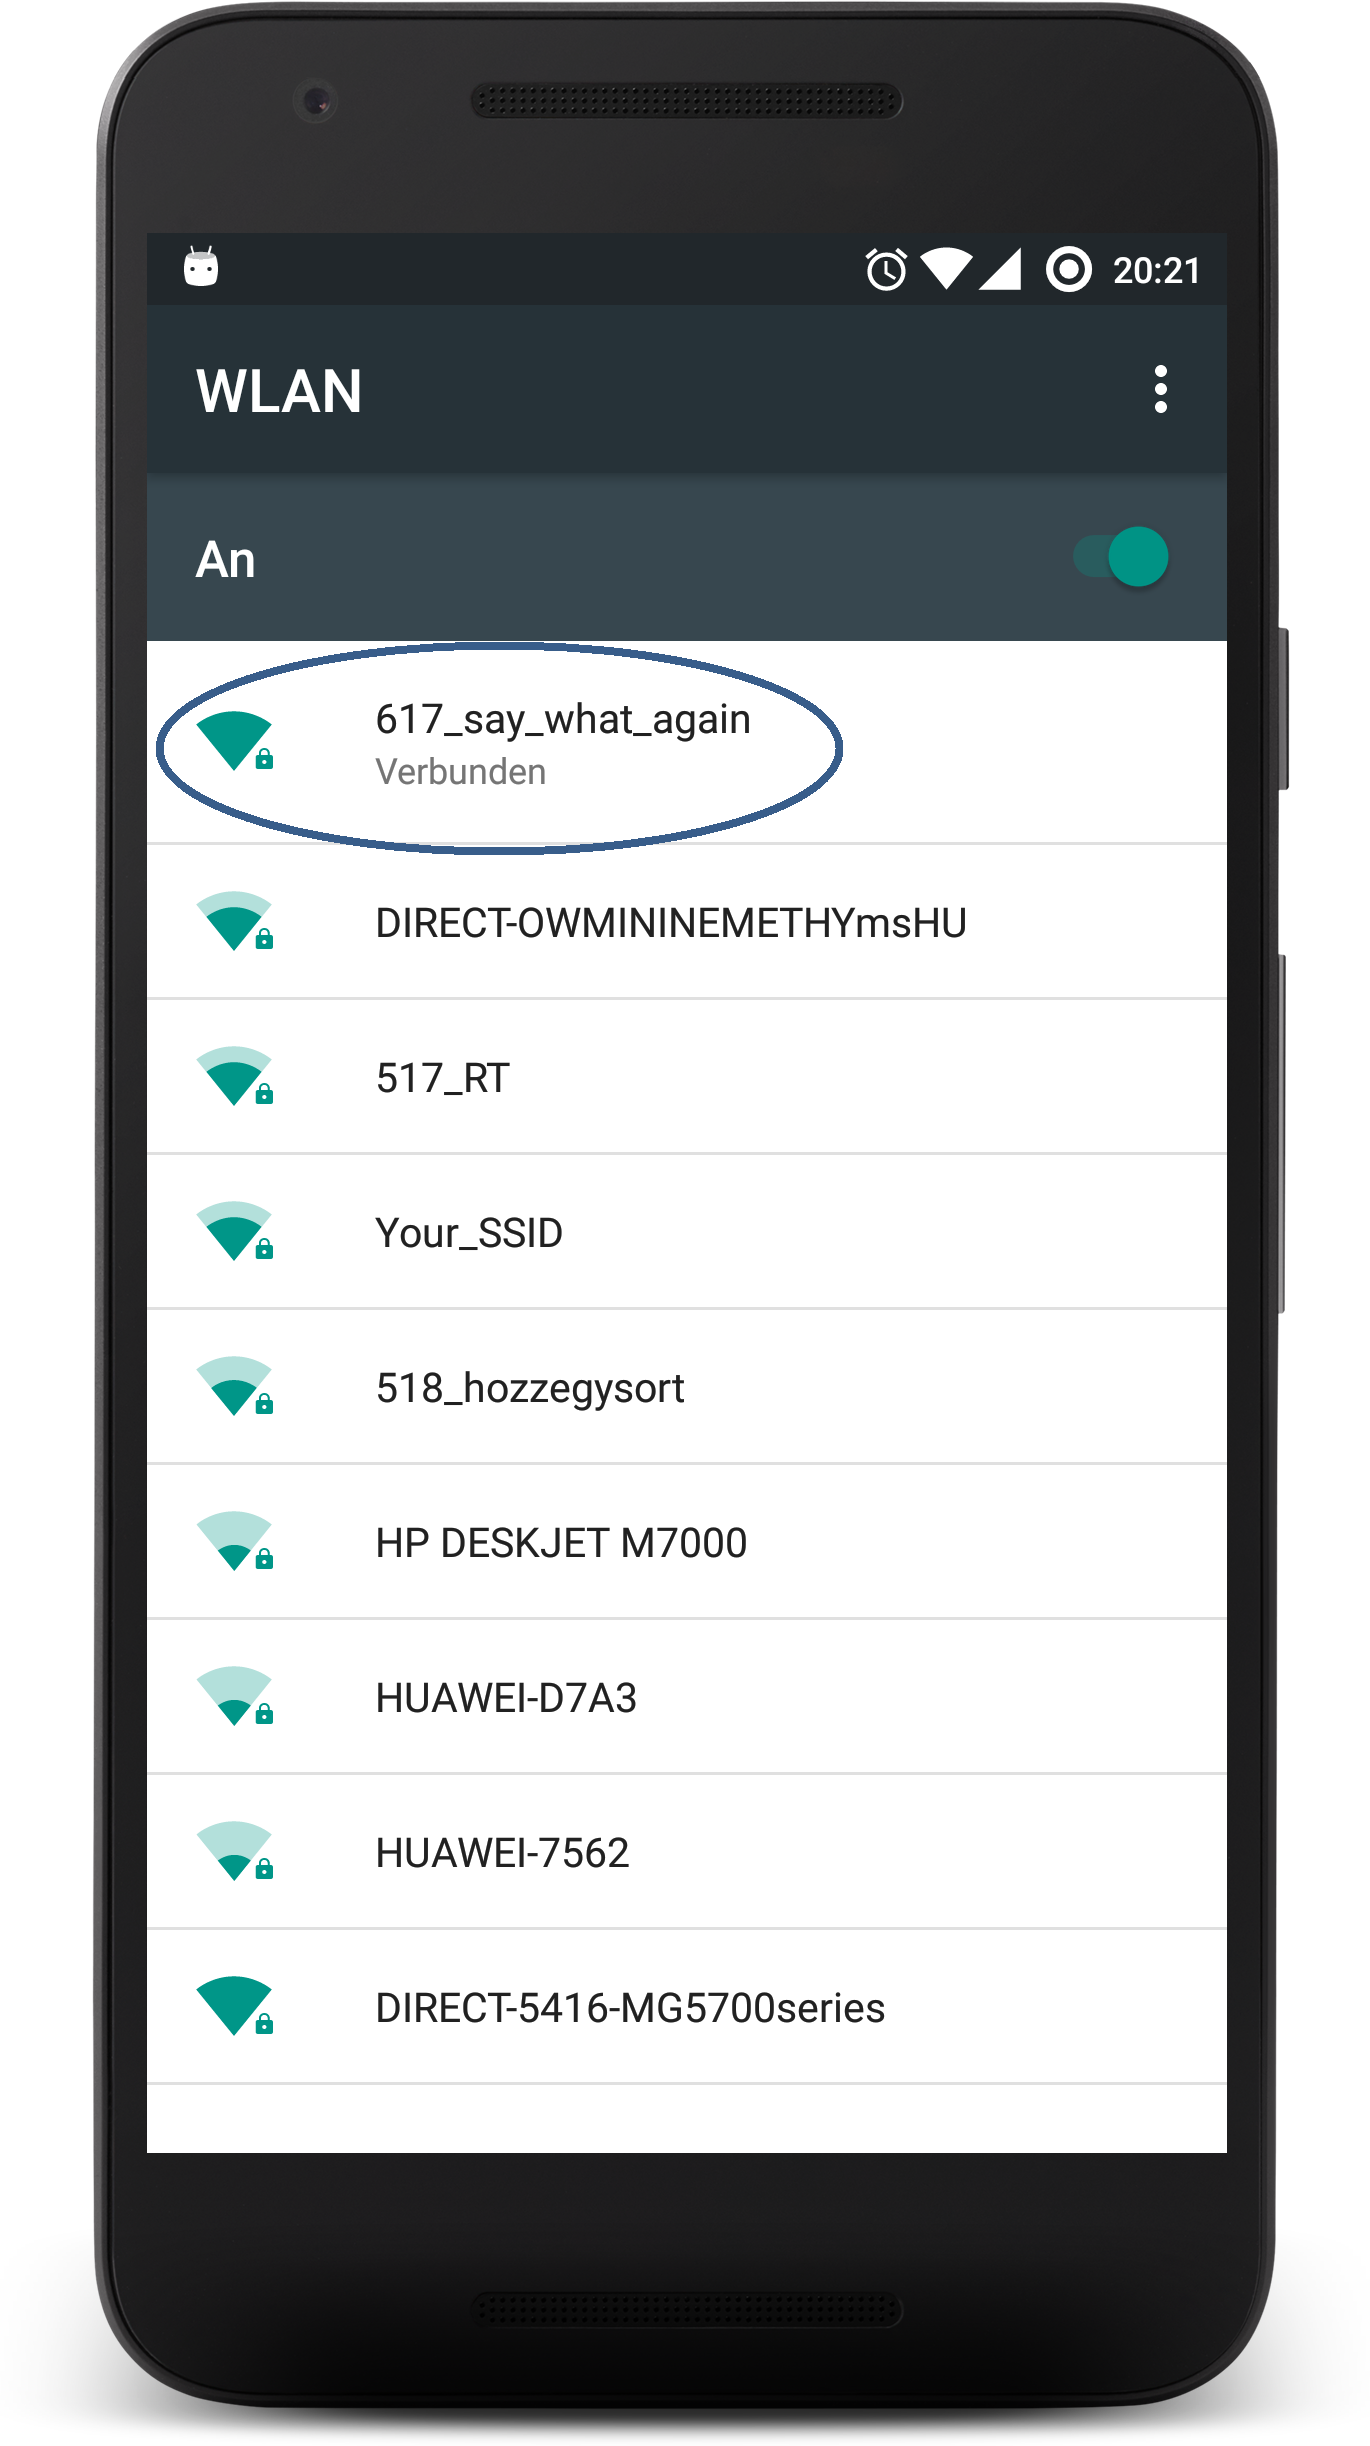
\includegraphics[width=5cm]{android_res/screen_pictures/wifi_err_03.png}
                \caption{Végül válaszza ki azt a hálózatot amire csatlakoztatva van a LED sor!}
                \label{fig:wifi_err_03}
            \end{figure}
        
        \subsubsection{Led sor IP-címének a beállítása}
            Először is szükségünk lesz a LED sor IP címére. Ezt két módon tehetjük meg:
            
            \begin{enumerate}
                \item Mobiltelefonunkon a Fing nevű alkalmazással könnyedén felderíthetjük a lokális Wifi hálózaton található eszközöket IP címükkel. Innen egyszerűen másoljuk ki vagy írjuk le egy papírlapra.
                \item A helyi hálózati routerre csatlakozott eszközök listájából
            \end{enumerate}
            
            \begin{figure}[!h]
                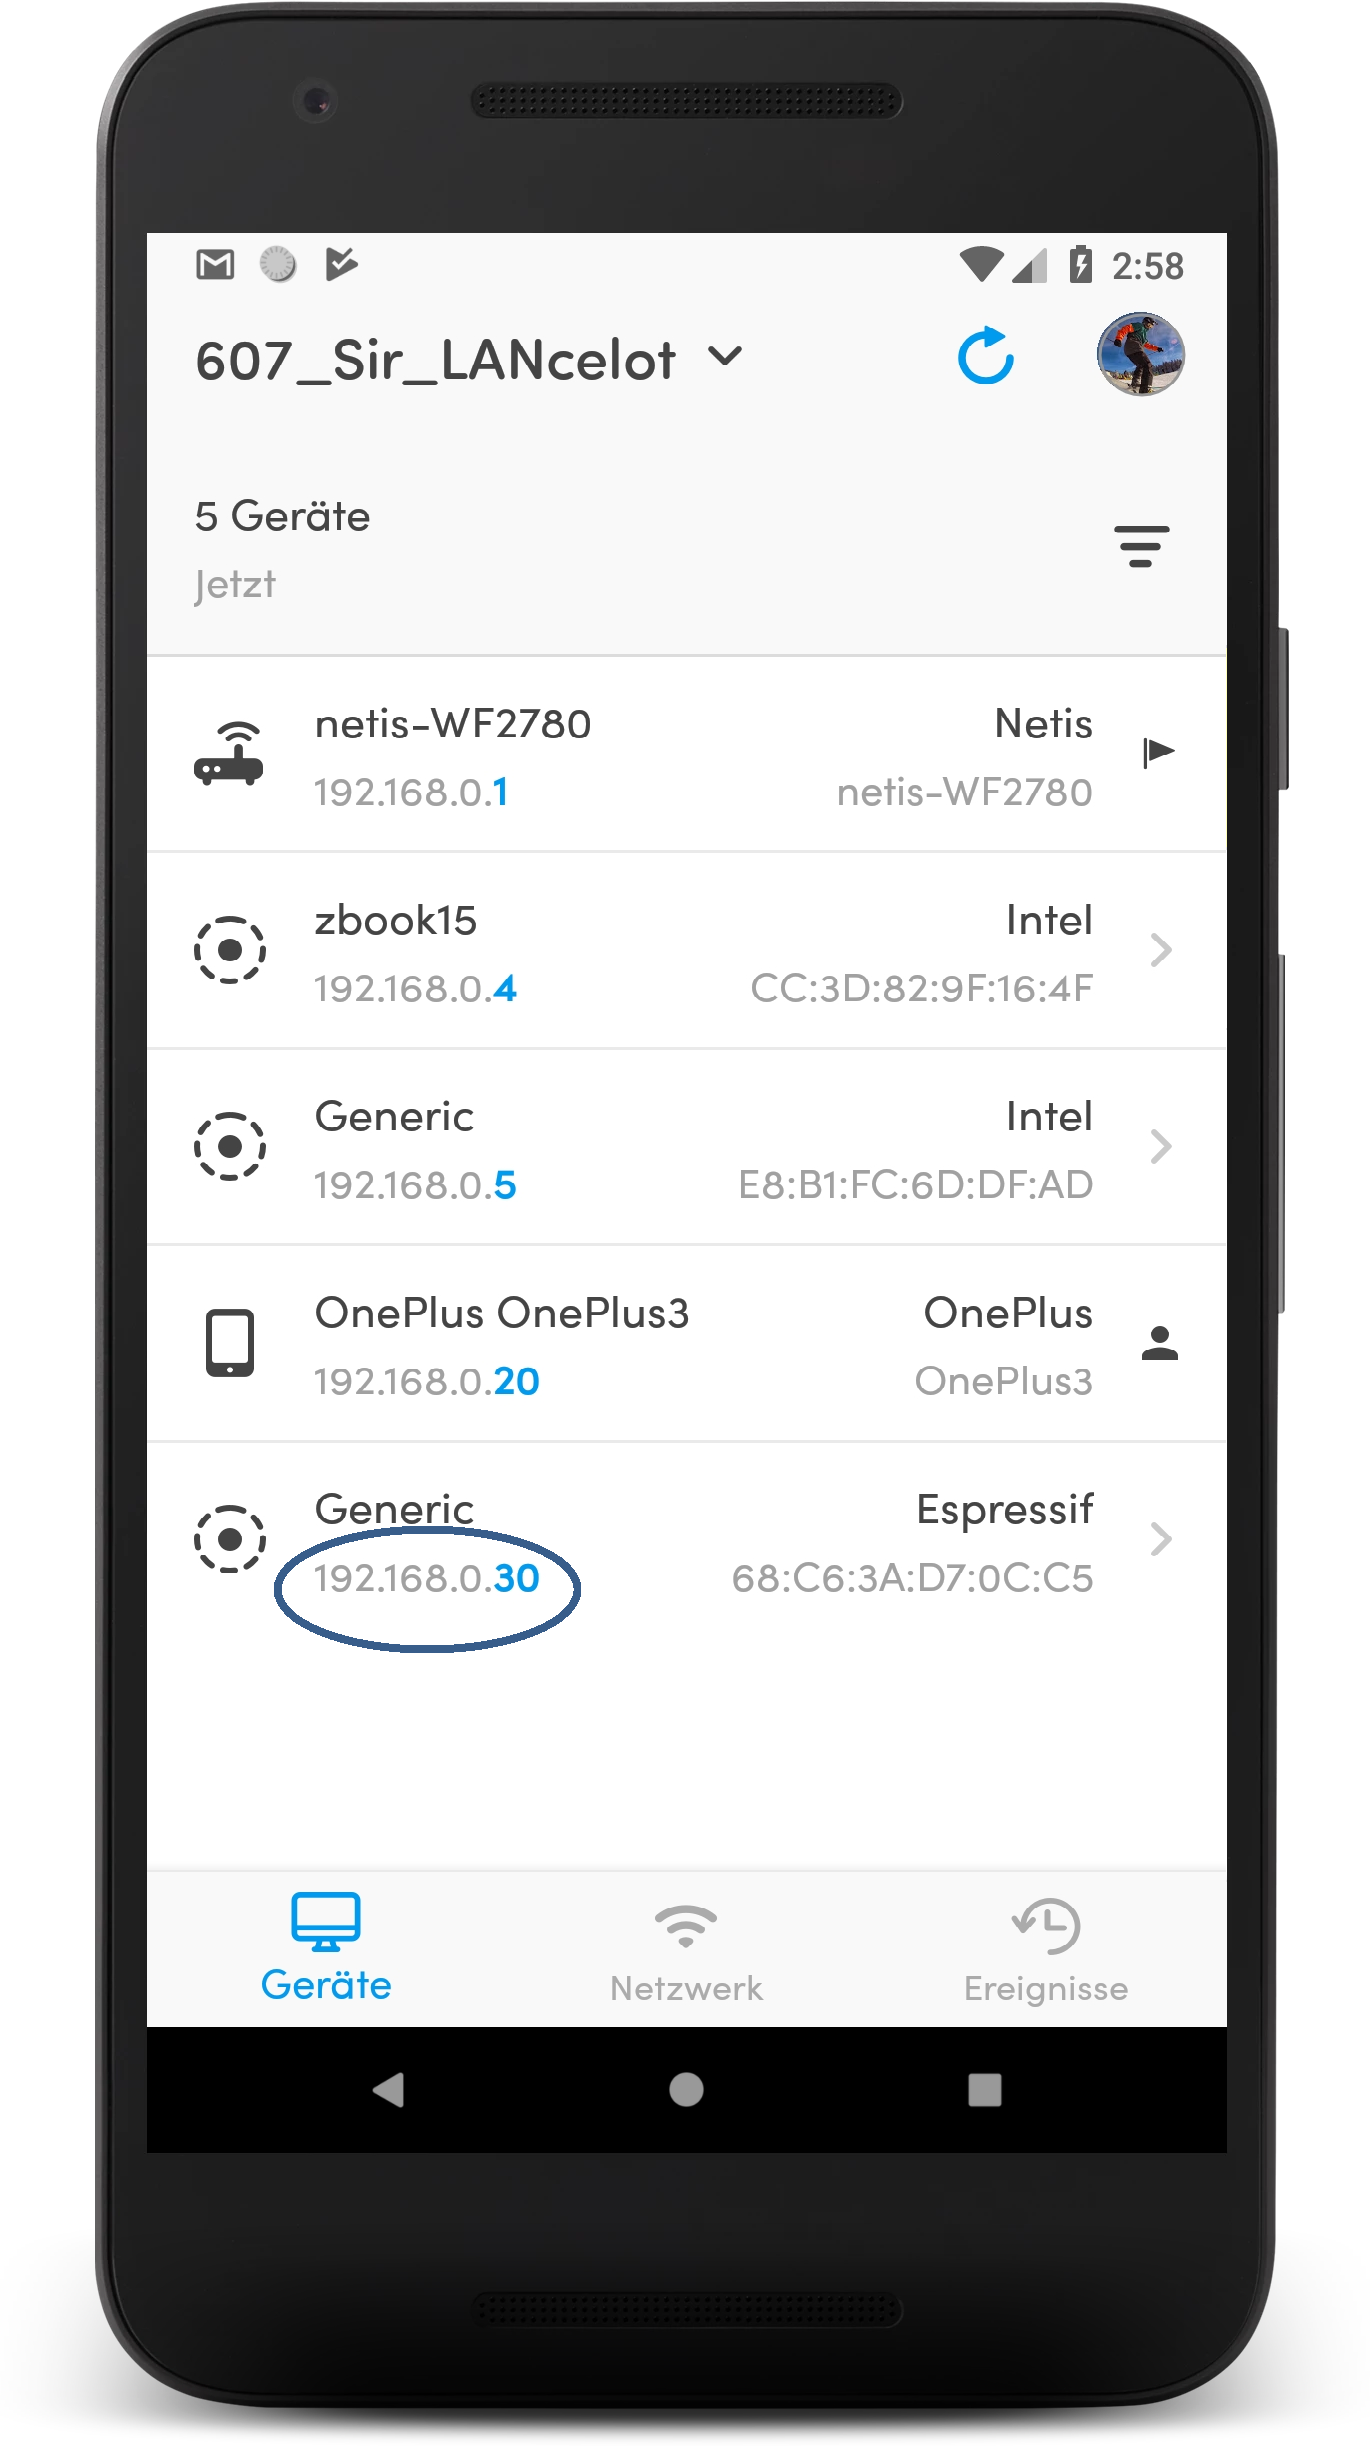
\includegraphics[height=7cm]{android_res/screen_pictures/ip_addr_fing}
                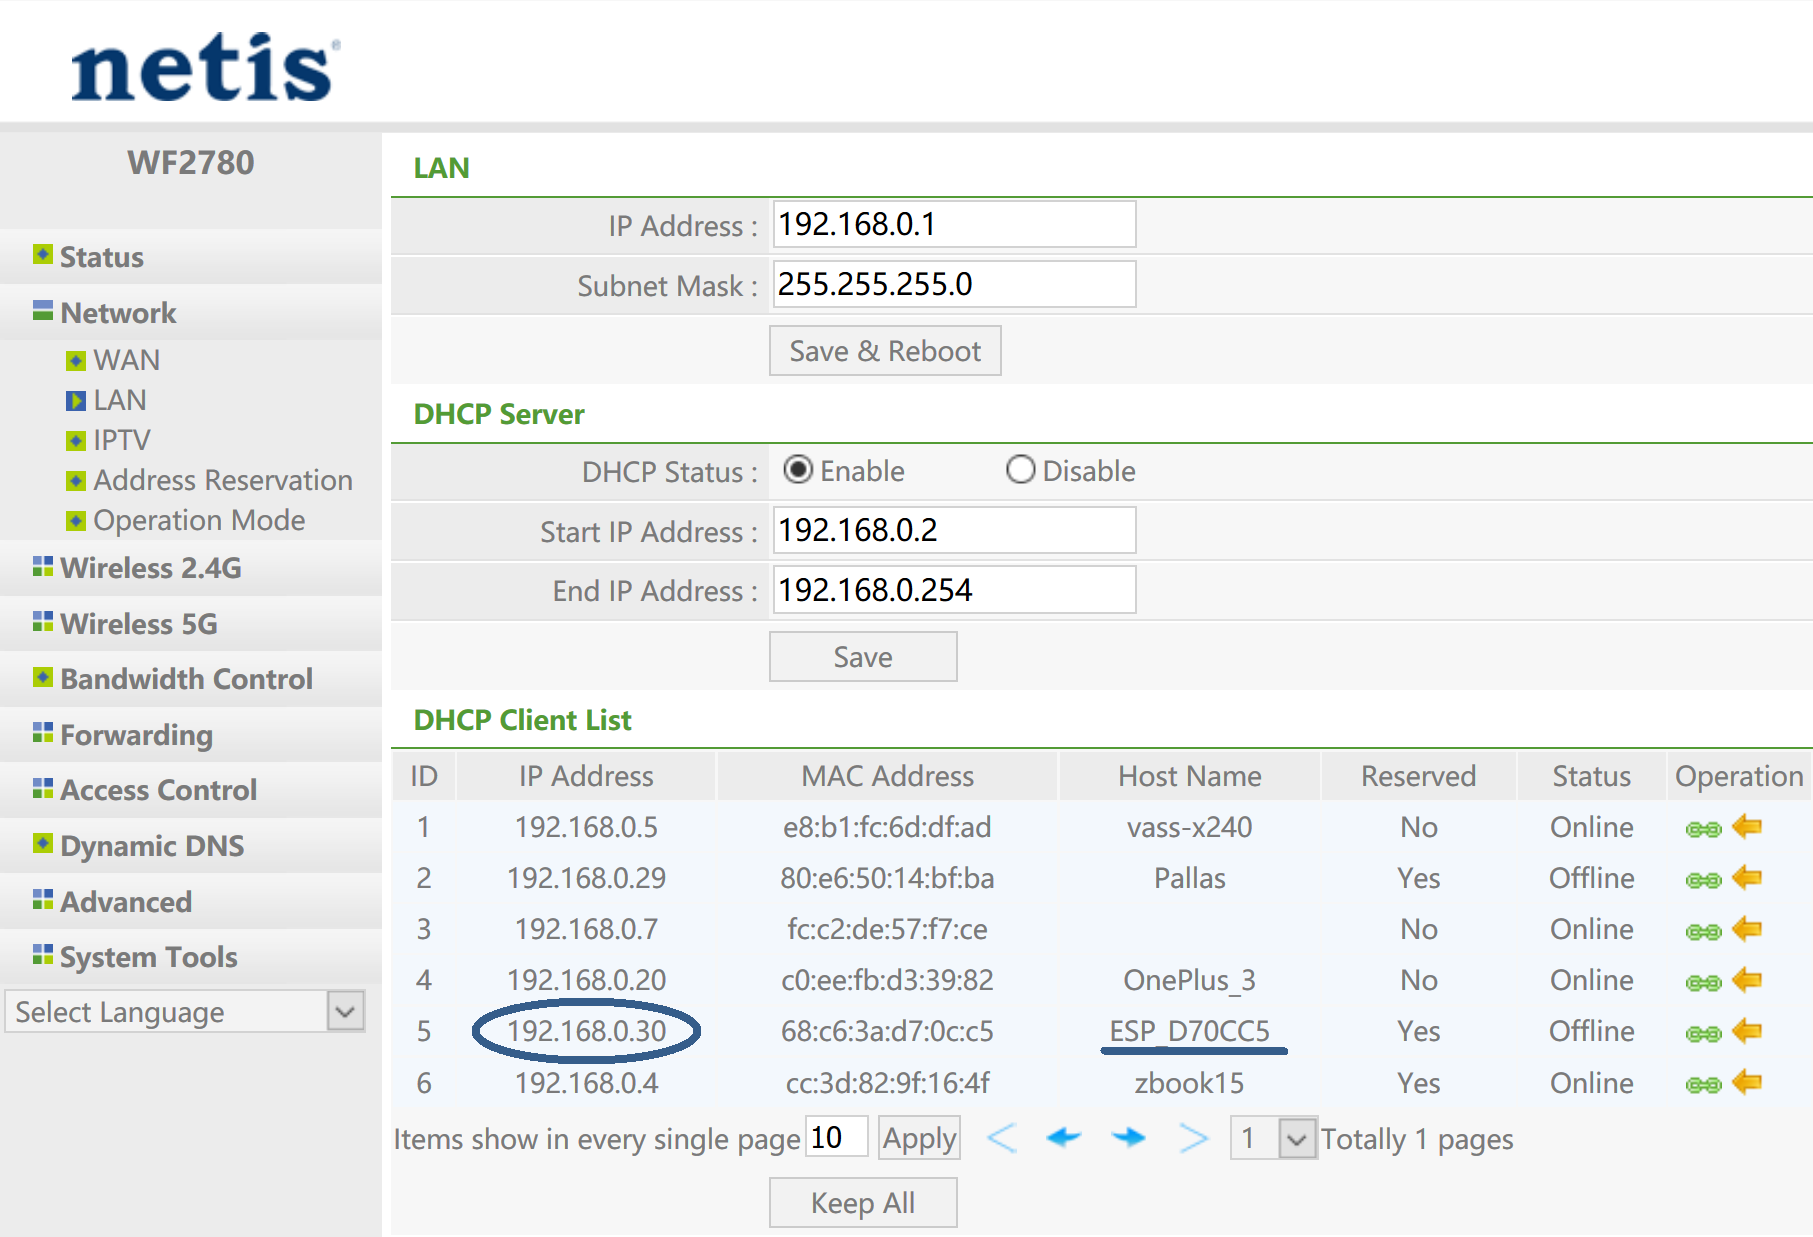
\includegraphics[height=7cm]{android_res/screen_pictures/ip_addr_router}
                \caption{LED sor IP címének felderítése Fing nevű alkalmazással és routerünk menüjéből}
            \end{figure}

            Ezek után visszalépve az alkalmazásba, átnavigálva a beállítások menüre beállíthatjuk a LED sor IP címét:
            
            \begin{enumerate}
                \item Navigációs menü előhozása
                
                    Az alkalmazáson belül bármelyik képernyőről ezzel (Ábra:  ~\ref{fig:onMenu1},~\ref{fig:onMenu2}) a két módszerrel lehet előhozni a navigációs menüt.
                    \begin{figure}[!h]
                        \begin{floatrow}
                            \ffigbox{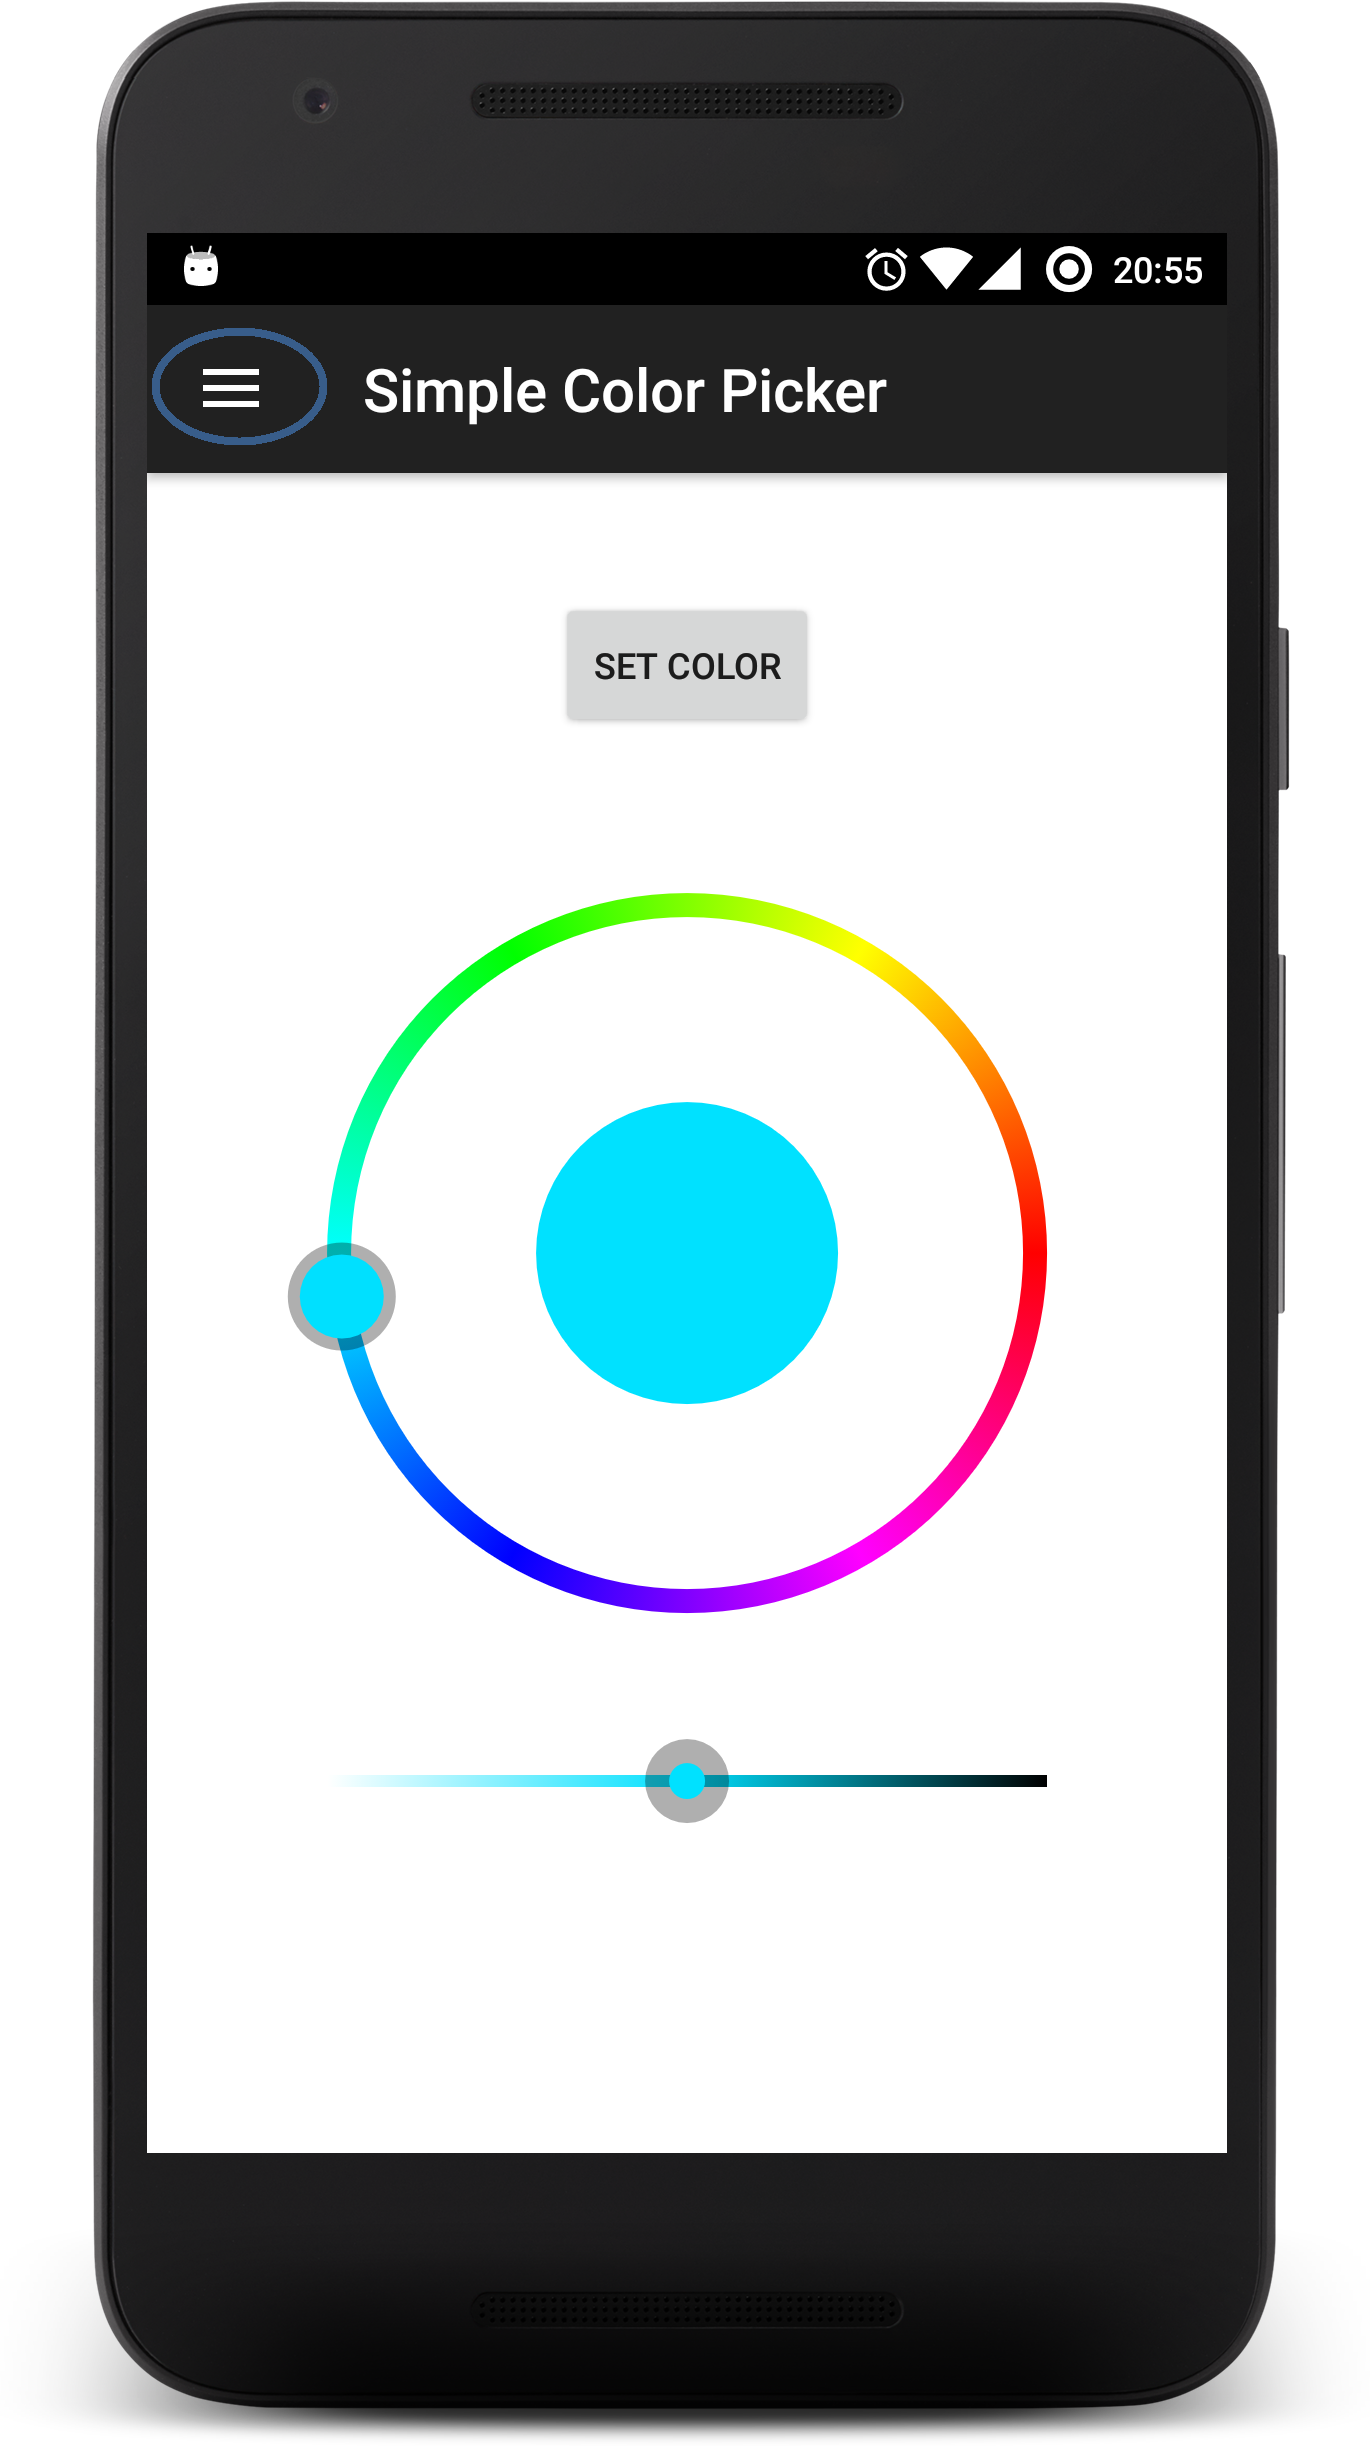
\includegraphics[width=5cm]{android_res/screen_pictures/nav_menu_01.png}}{\caption{A menü gombra való kattintással}\label{fig:onMenu1}}
                            \ffigbox{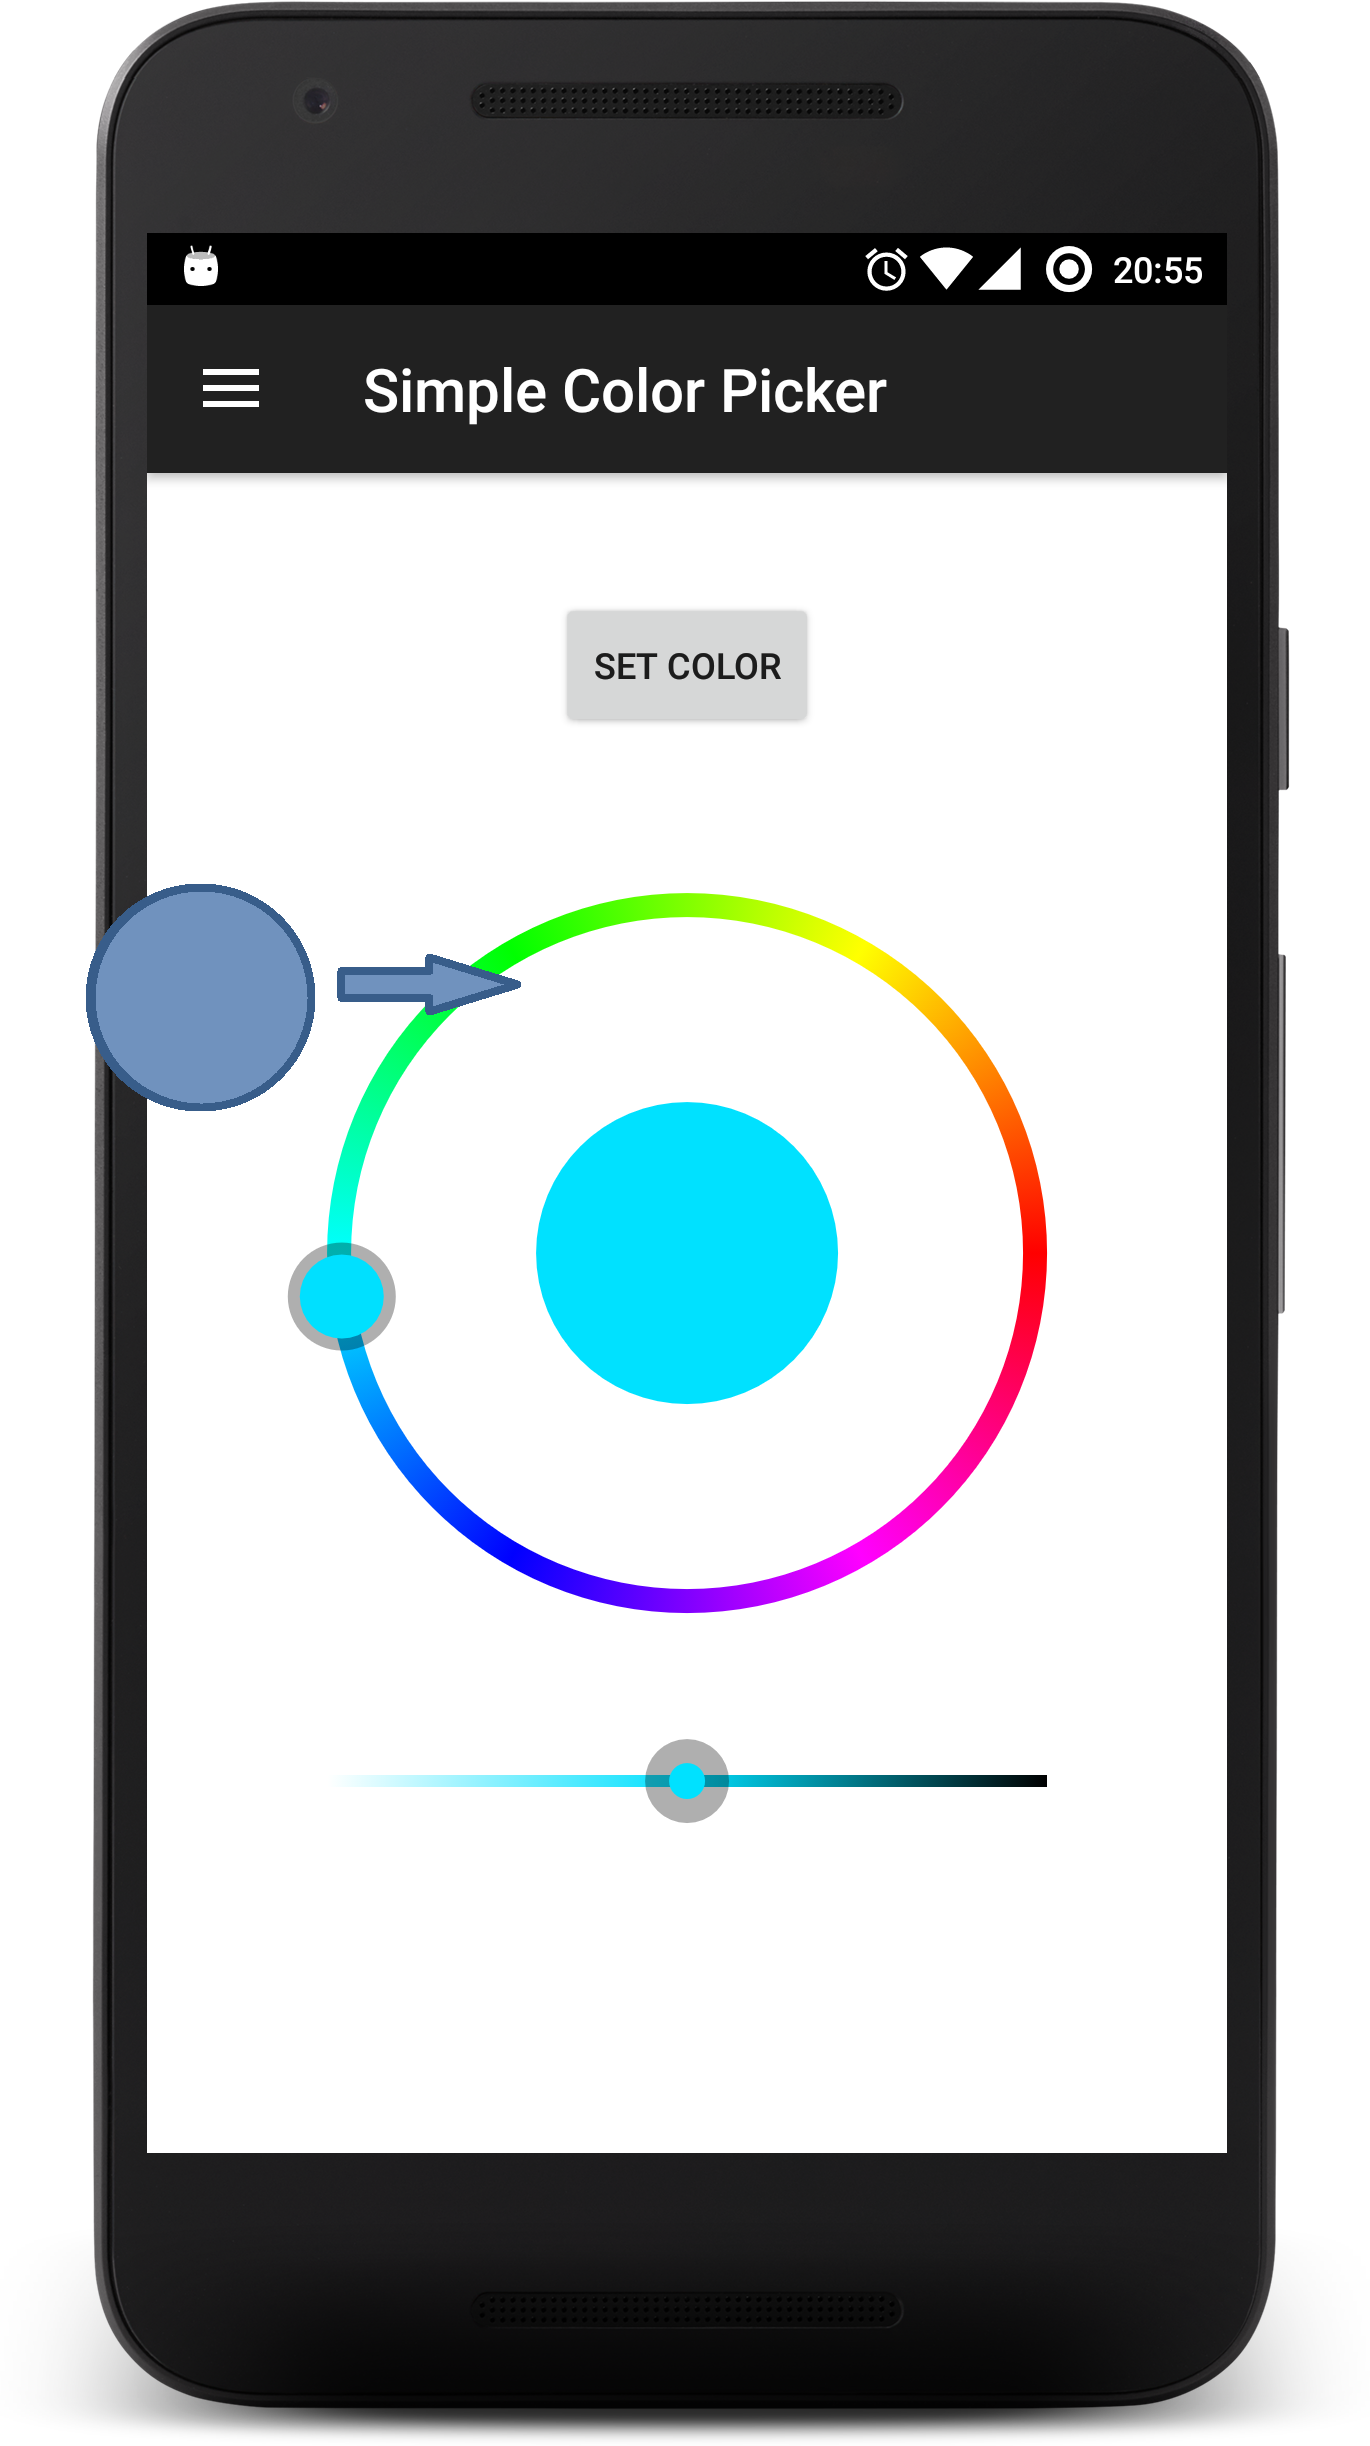
\includegraphics[width=5cm]{android_res/screen_pictures/nav_menu_02.png}}{\caption{˝Swipe gesture segítségével˝}\label{fig:onMenu2}}
                        \end{floatrow}
                    \end{figure}\\
                    
                \item Beállítások fül kiválasztása
                     \begin{figure}[!h]
                        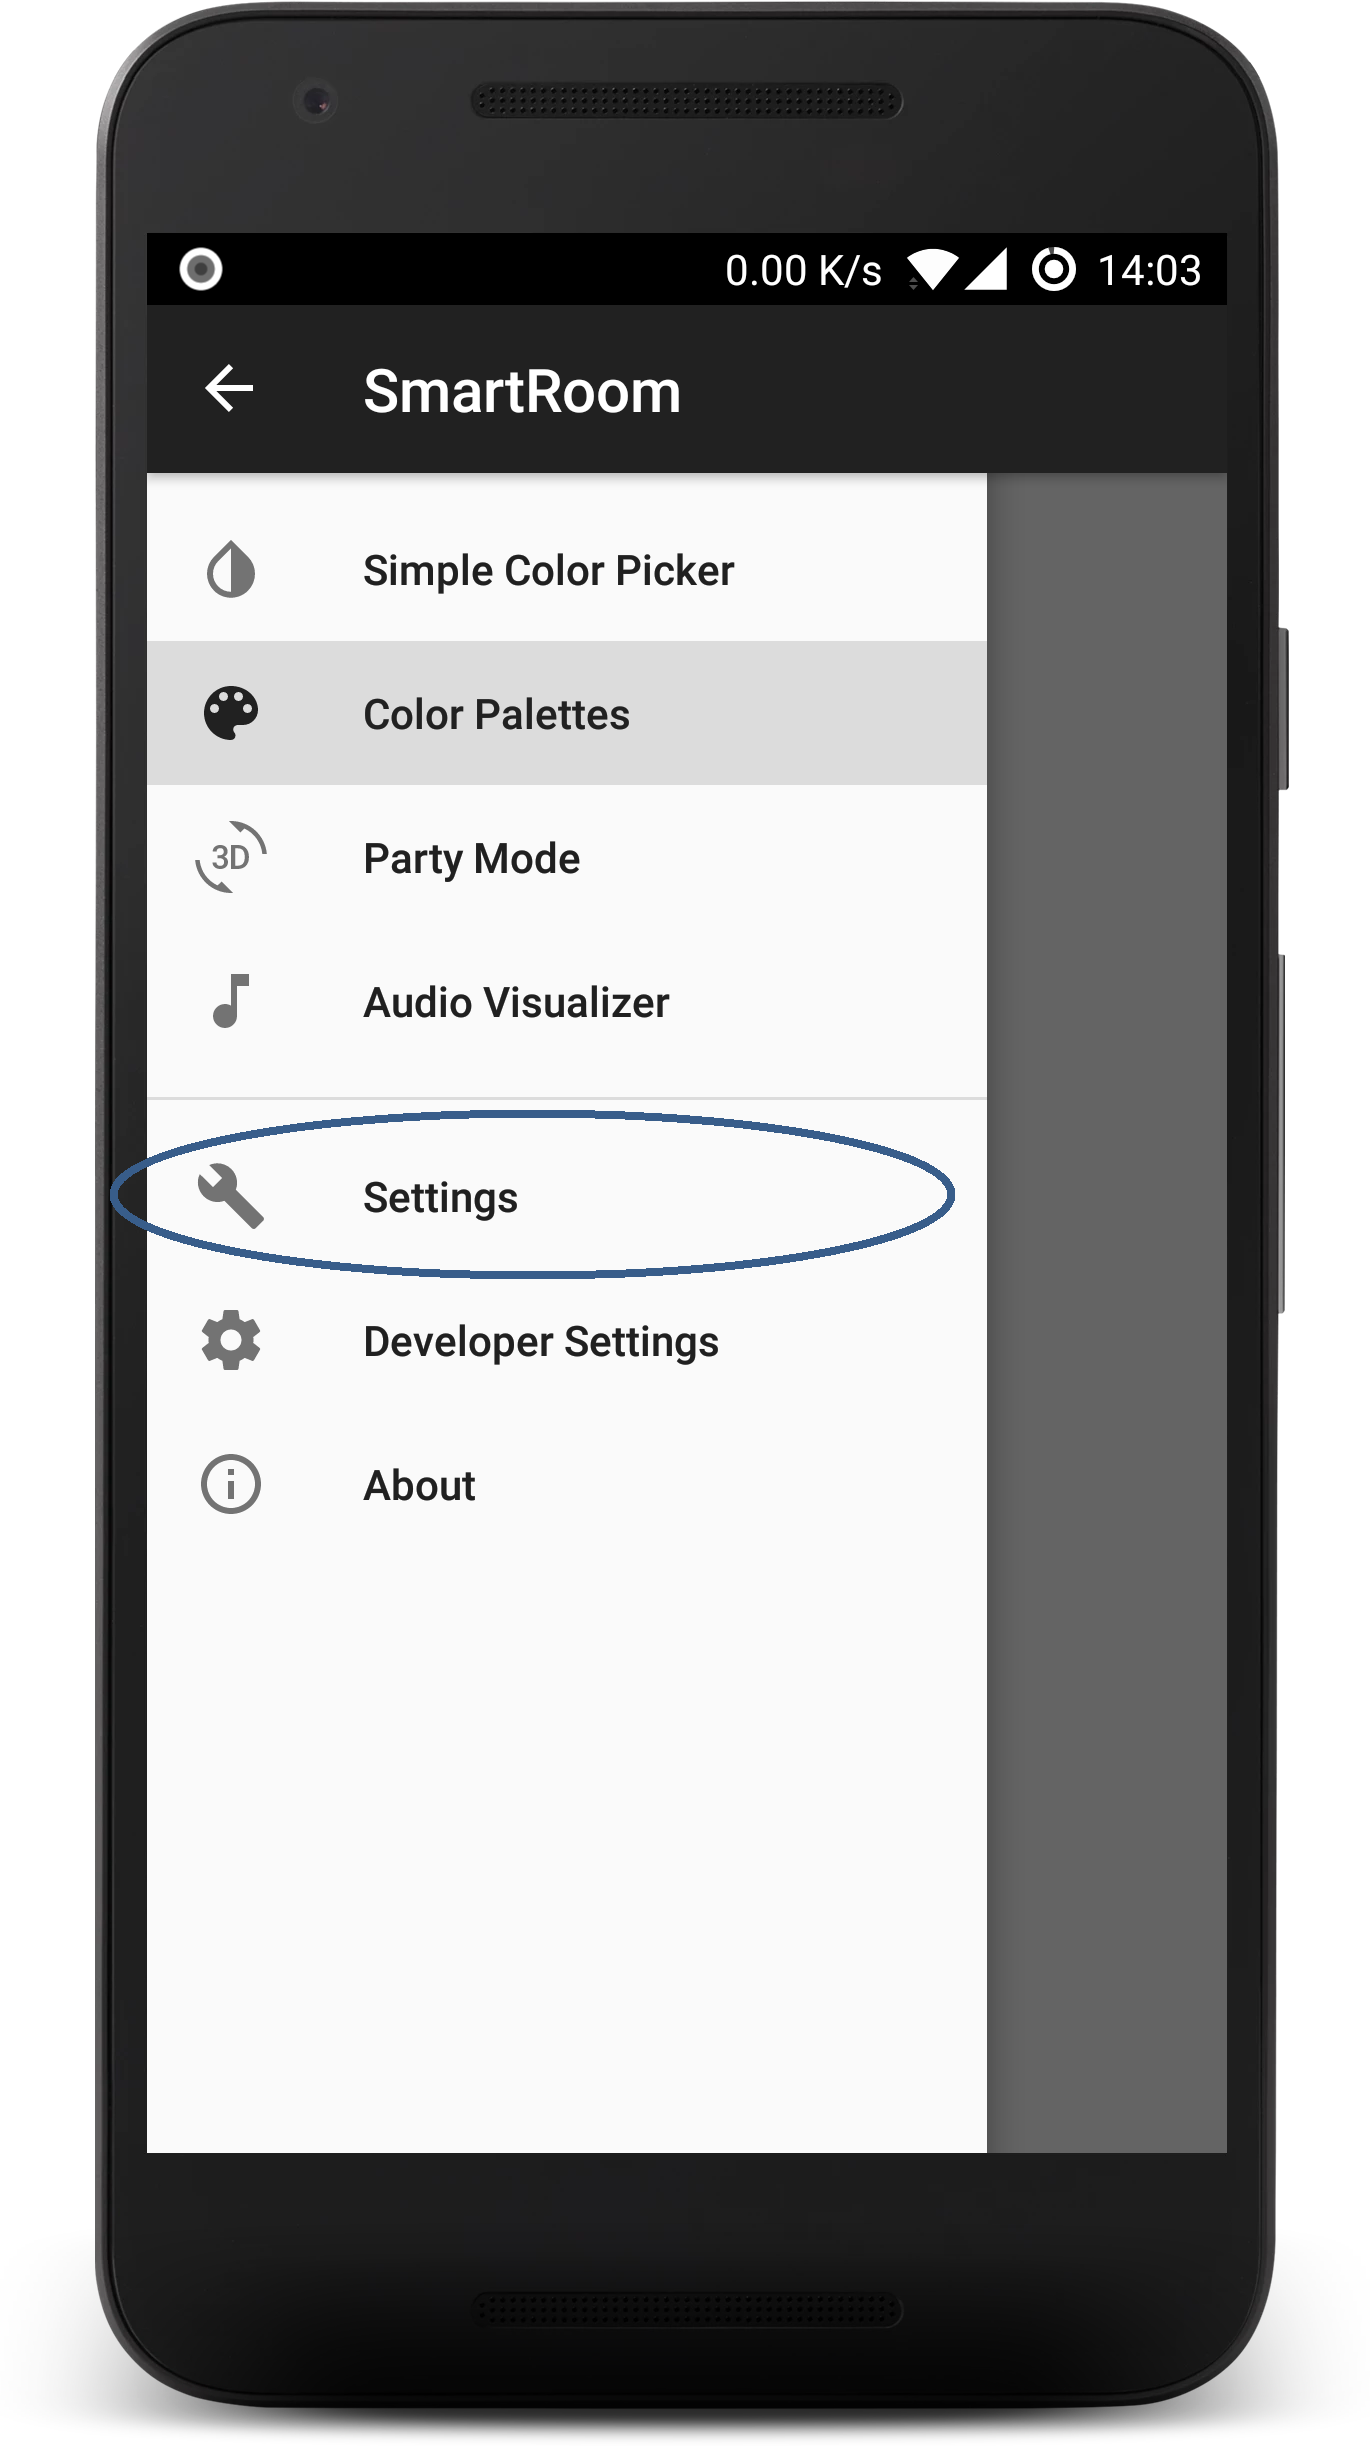
\includegraphics[height=7cm]{android_res/screen_pictures/tap_settings_menu}
                        \caption{Koppintson a Beállítások fülre! //TODO}
                    \end{figure}
                    
                \item Helyi hálózati IP cím beállítása (Ábra: ~\ref{fig:tap_local_ip},~\ref{fig:set_local_ip})
                    \begin{figure}[h!]
                        \begin{floatrow}
                            \ffigbox{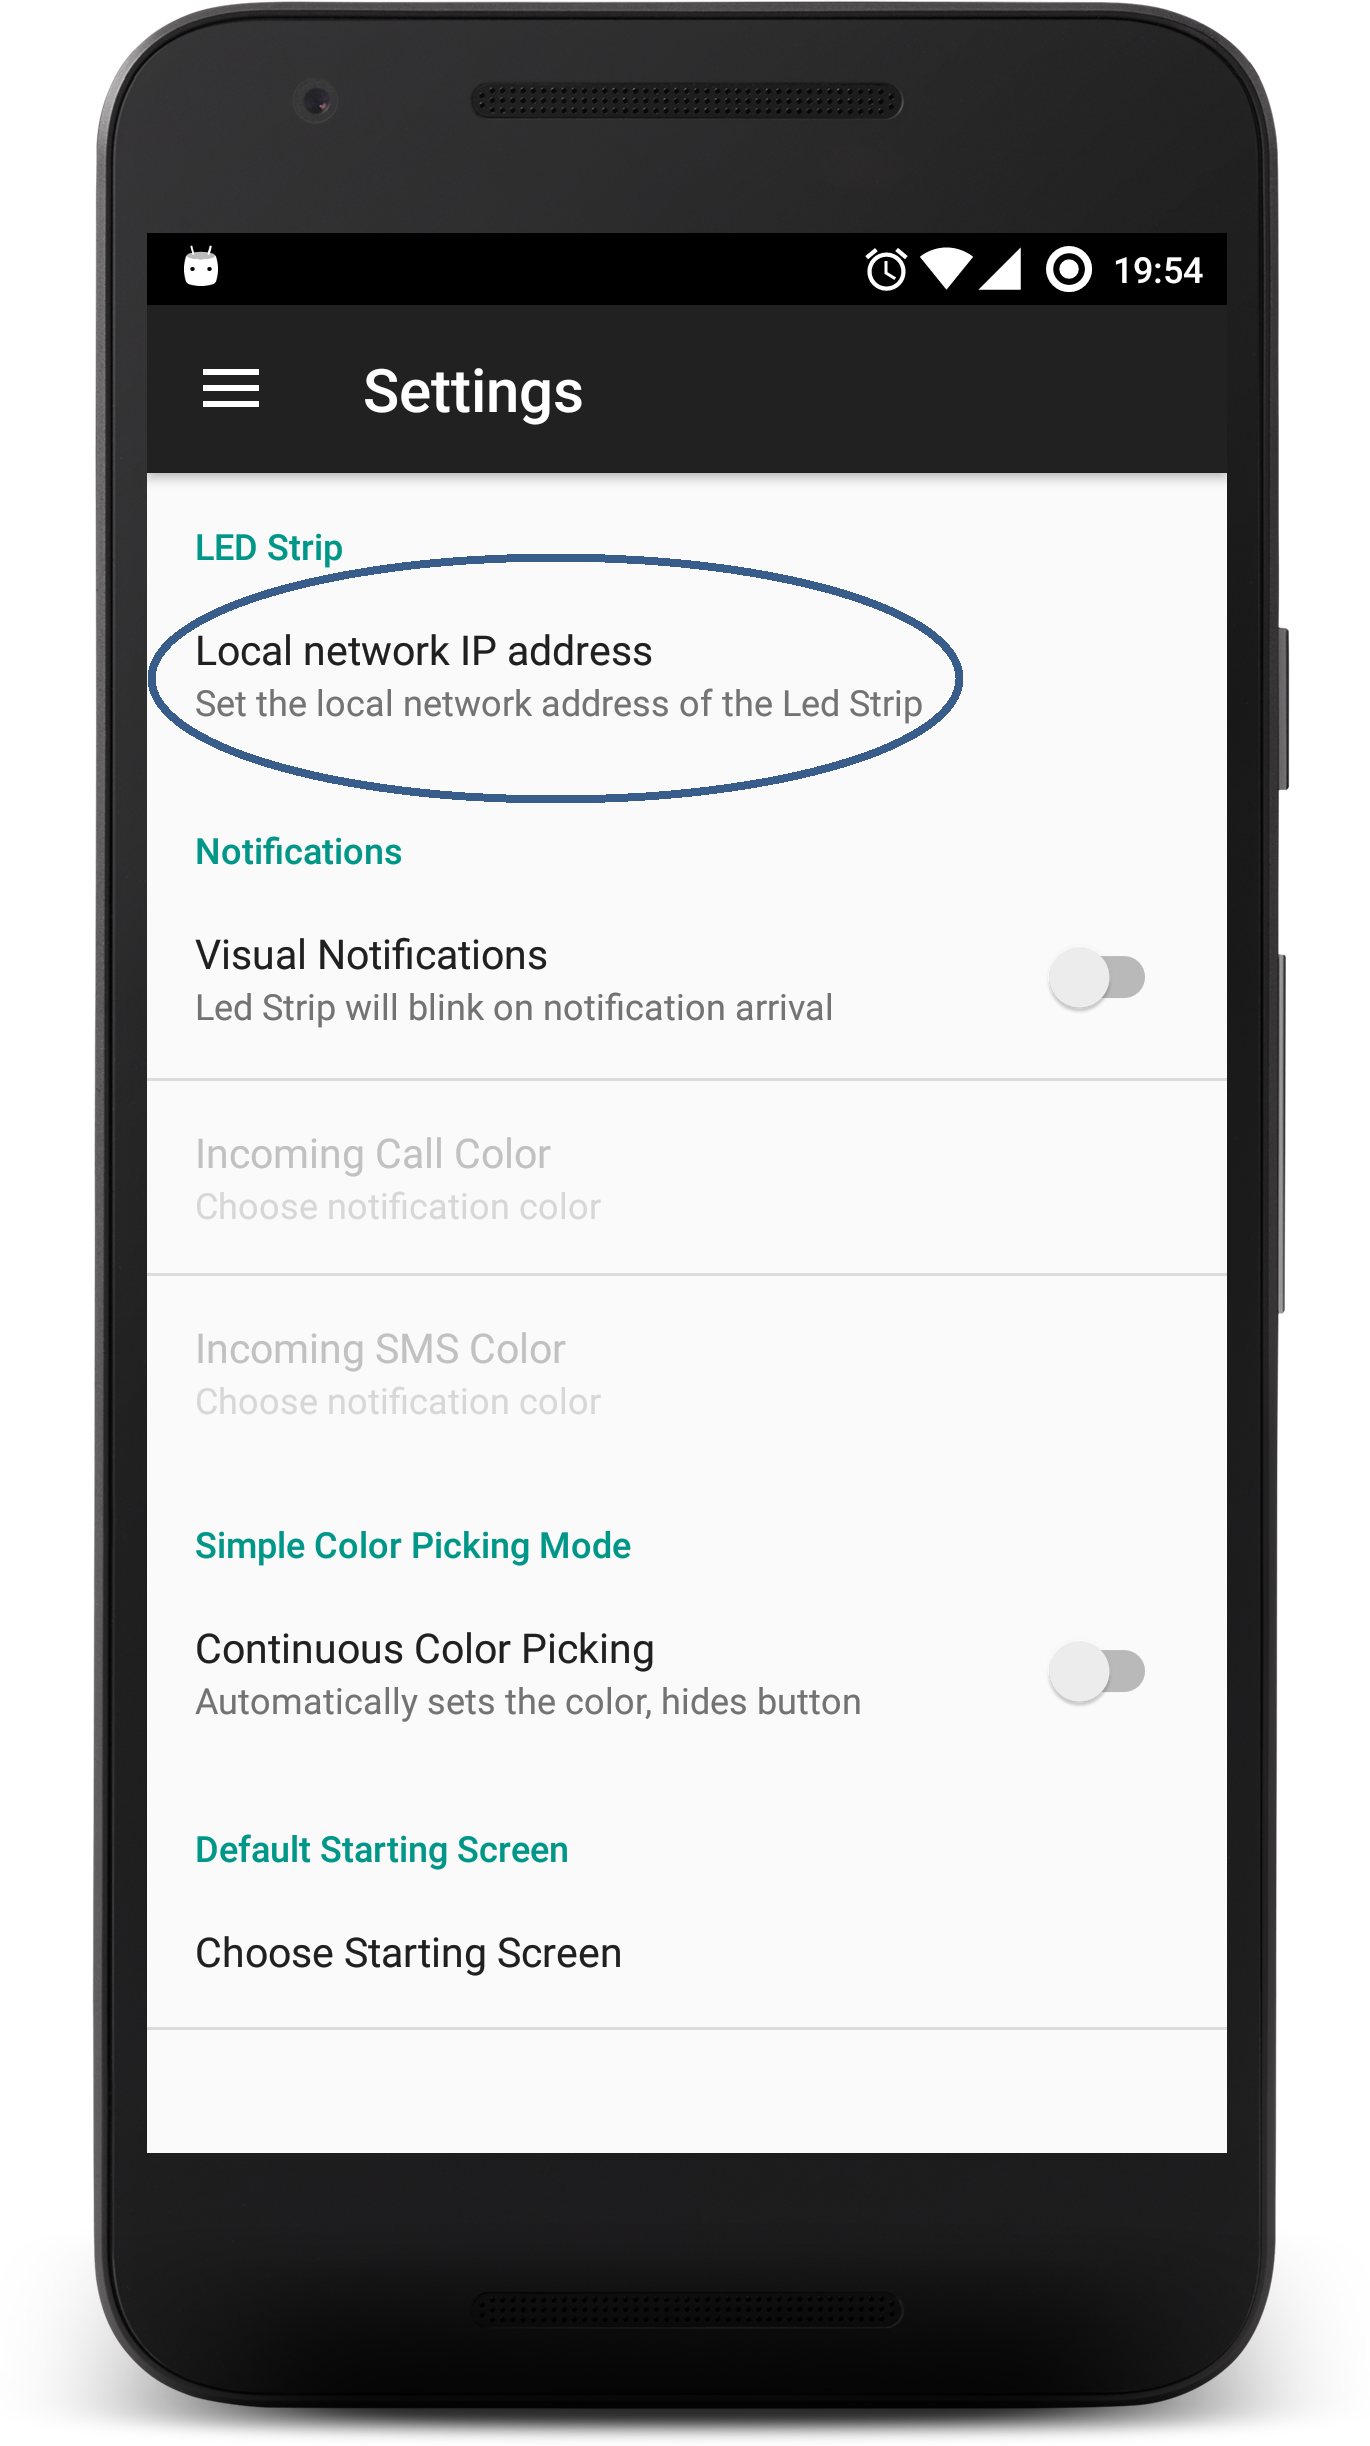
\includegraphics[width=5cm]{android_res/screen_pictures/tap_local_ip.png}}{\caption{Koppintson a helyi hálózati IP cím beállításra!}\label{fig:tap_local_ip}}
                            \ffigbox{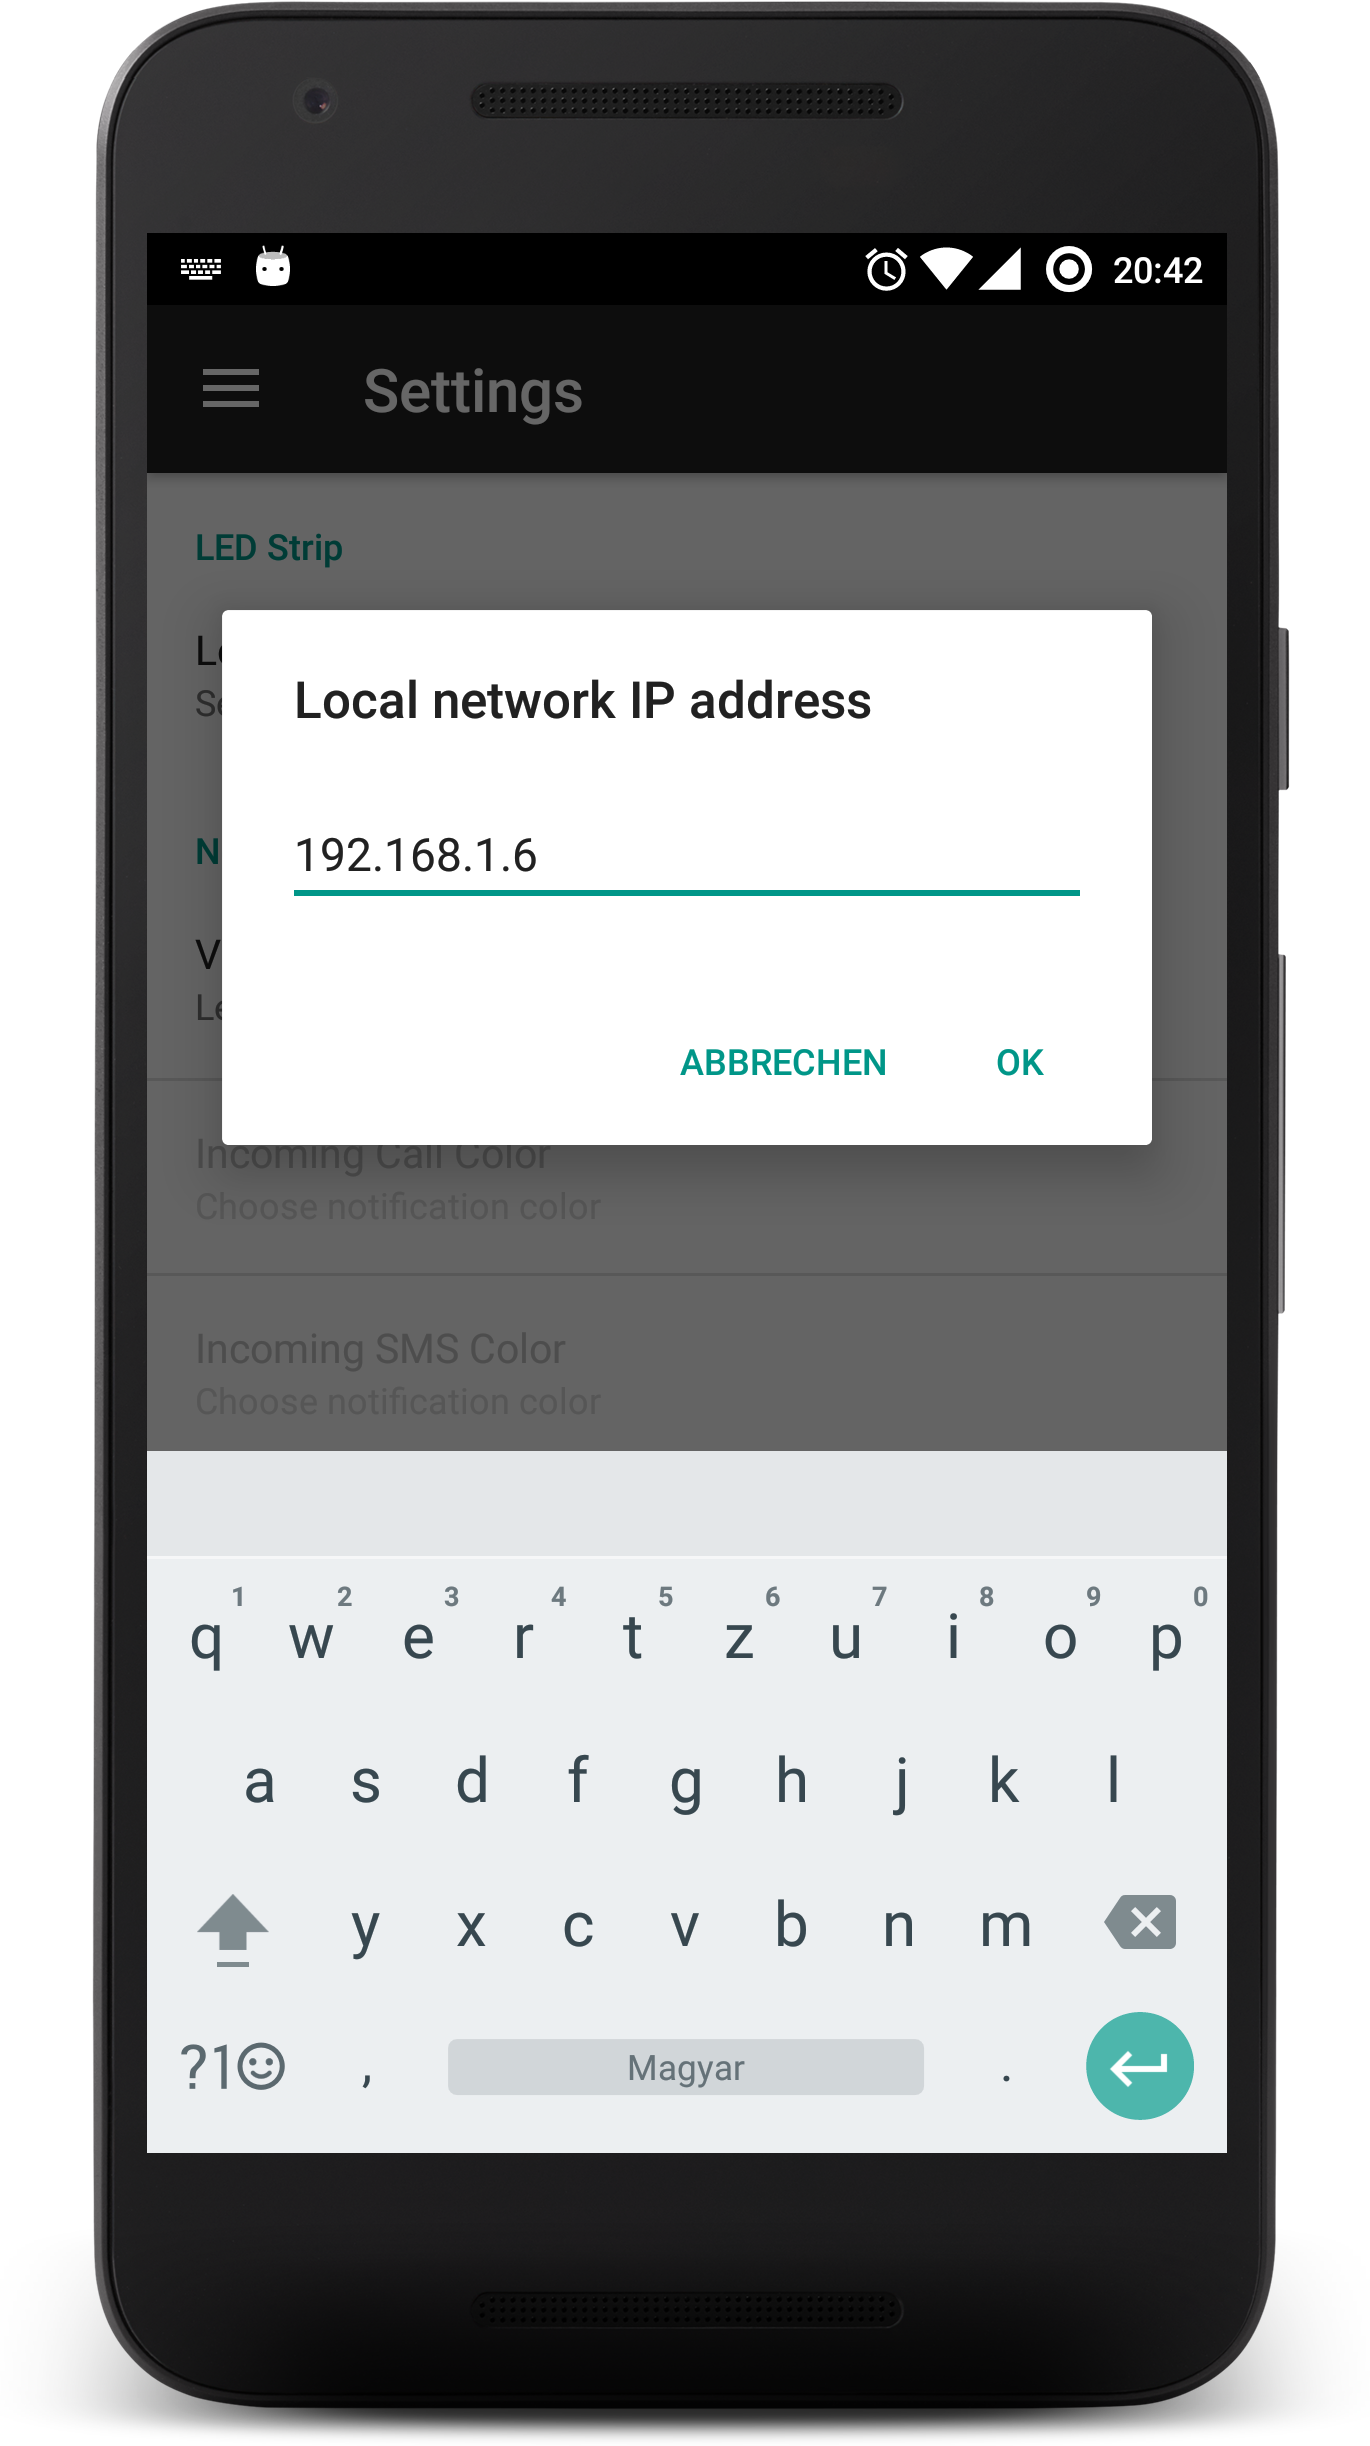
\includegraphics[width=5cm]{android_res/screen_pictures/set_local_ip.png}}{\caption{Állítsa be az IP címet, majd koppintson
az Ok gombra!}\label{fig:set_local_ip}}
                        \end{floatrow}
                    \end{figure}
                
            \end{enumerate}
            
            
        
%https://shop.technexion.com/pico-pi-imx7-startkit-rainbow-hat.html
%https://developer.android.com/about/
        \subsubsection{Simple Color Picker mód} %https://github.com/LarsWerkman/HoloColorPicker
            Ezen a képernyőn egy külső forrásból származó Color Picker található. A csúszkák mozgatásával tudjuk kiválasztani az adot színt, majd a \textit{Szín beállítása} gomb megnyomásával állíthatjuk be a LED sor színét (Ábra ~\ref{fig:s_cp_01},~\ref{fig:s_cp_02}).
            
            \begin{figure}[h!]
                \begin{floatrow}
                    \ffigbox{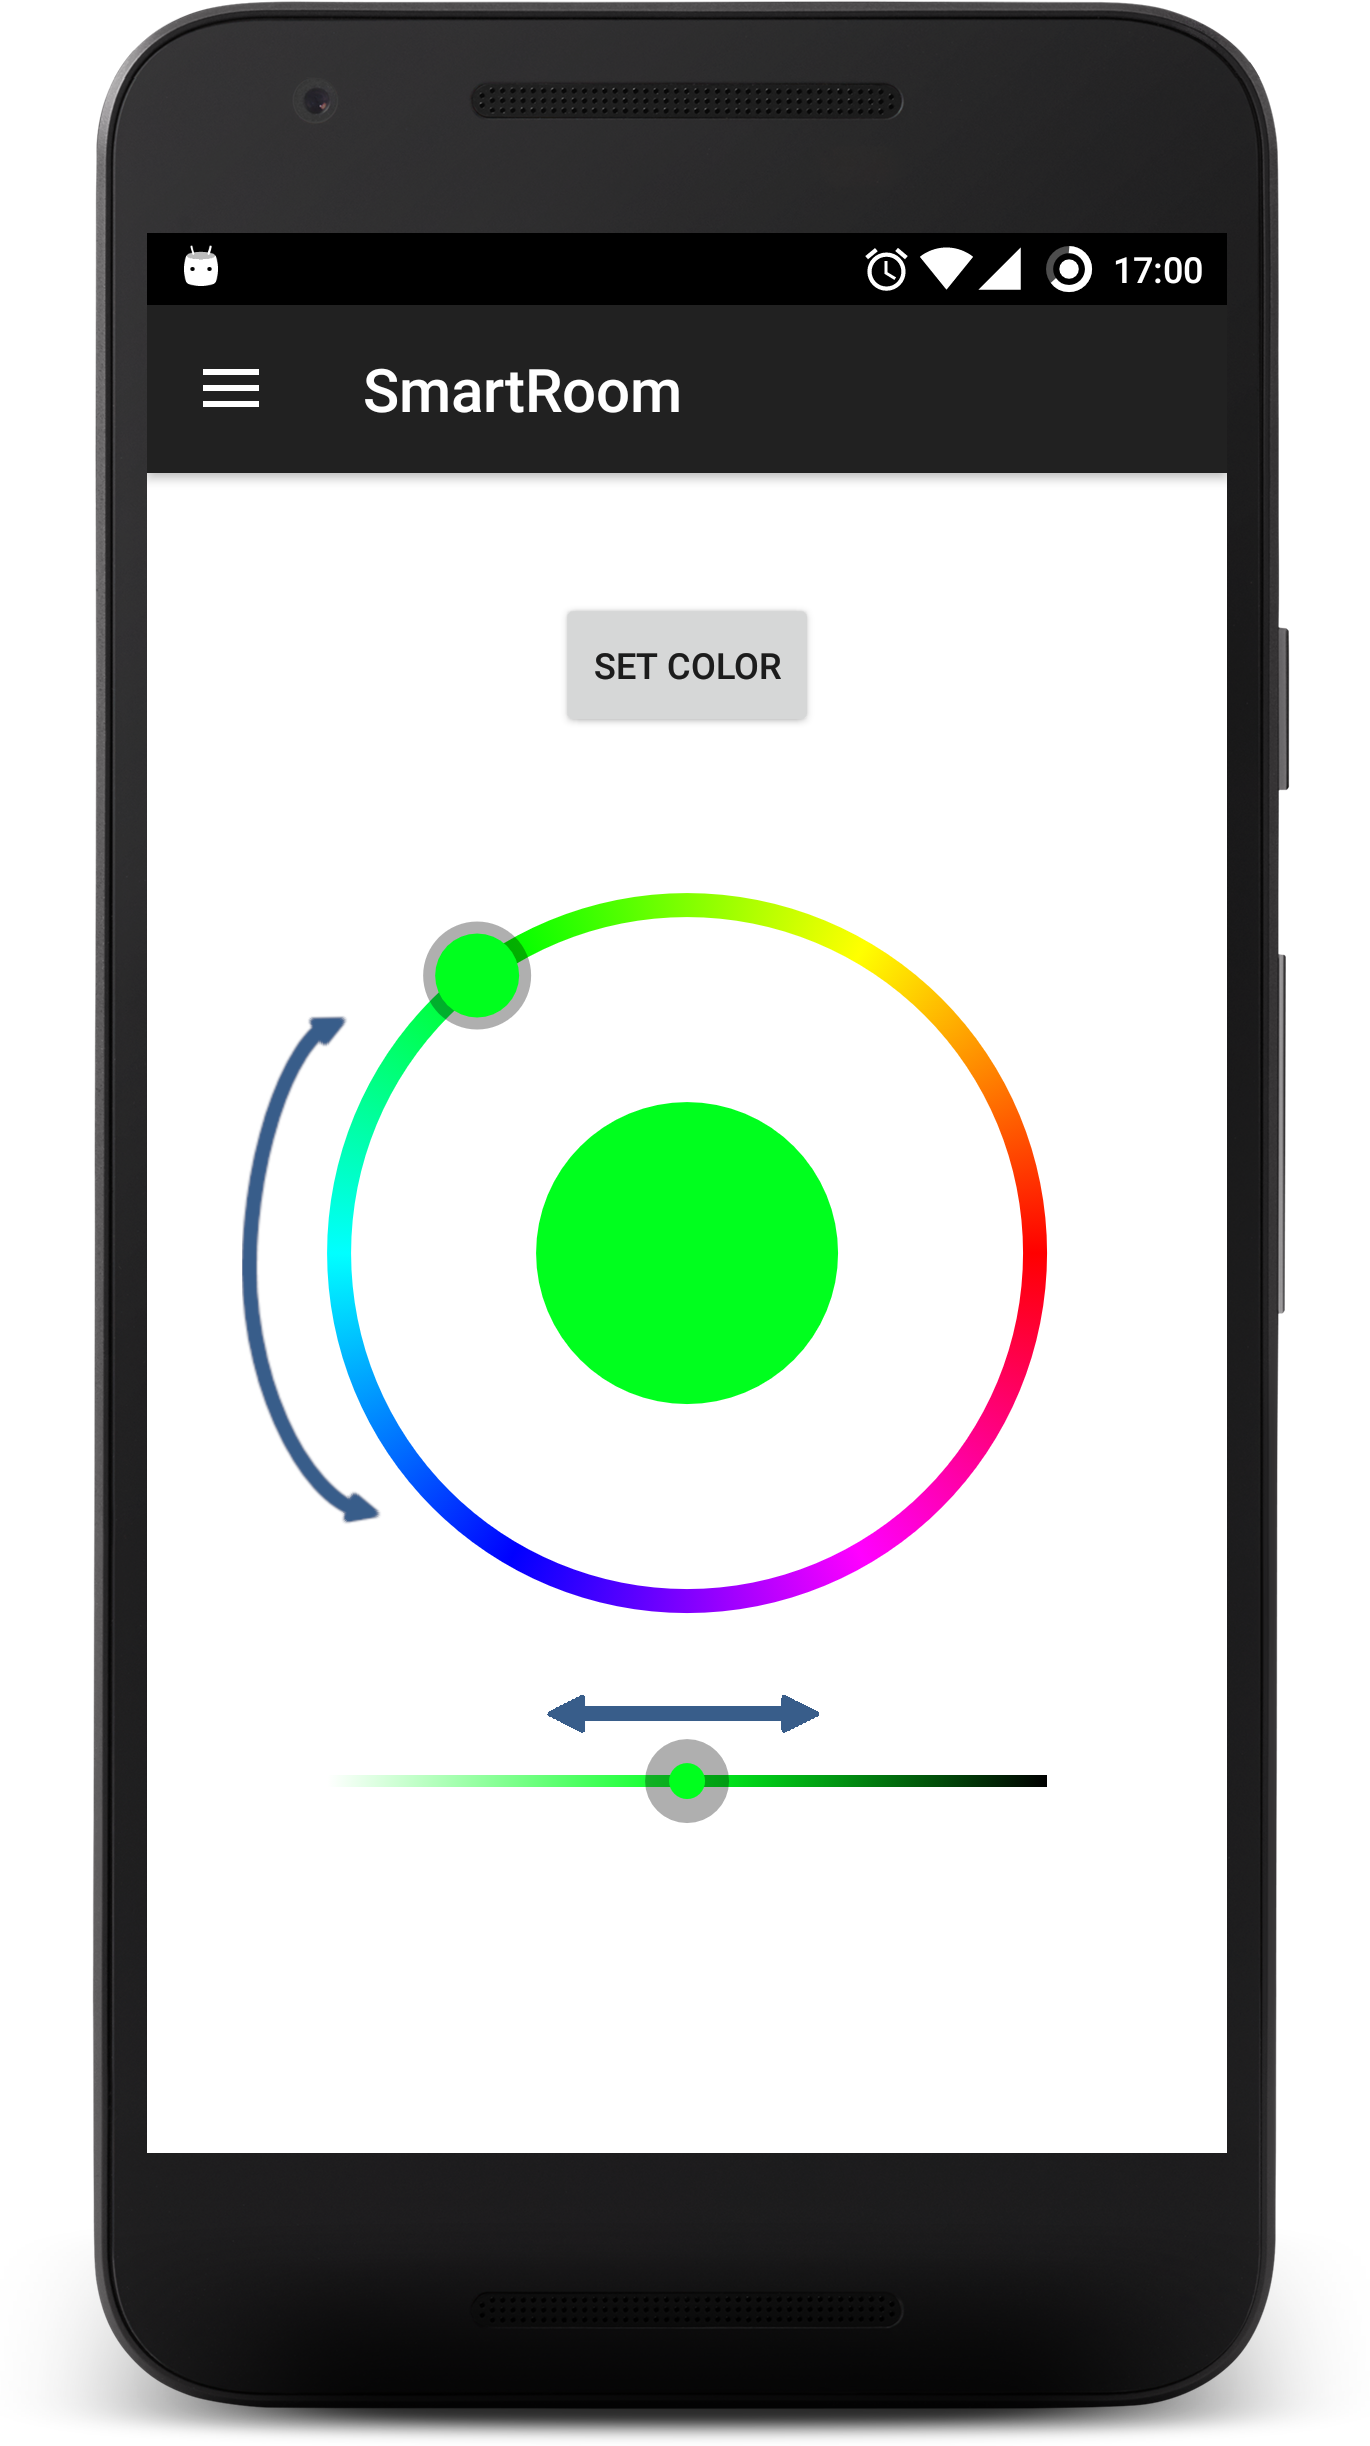
\includegraphics[width=5cm]{android_res/screen_pictures/s_cp_01.png}}{\caption{A csúszkák mozgatásával változtathatjuk a megjelenítendő színt}\label{fig:s_cp_01}}
                    \ffigbox{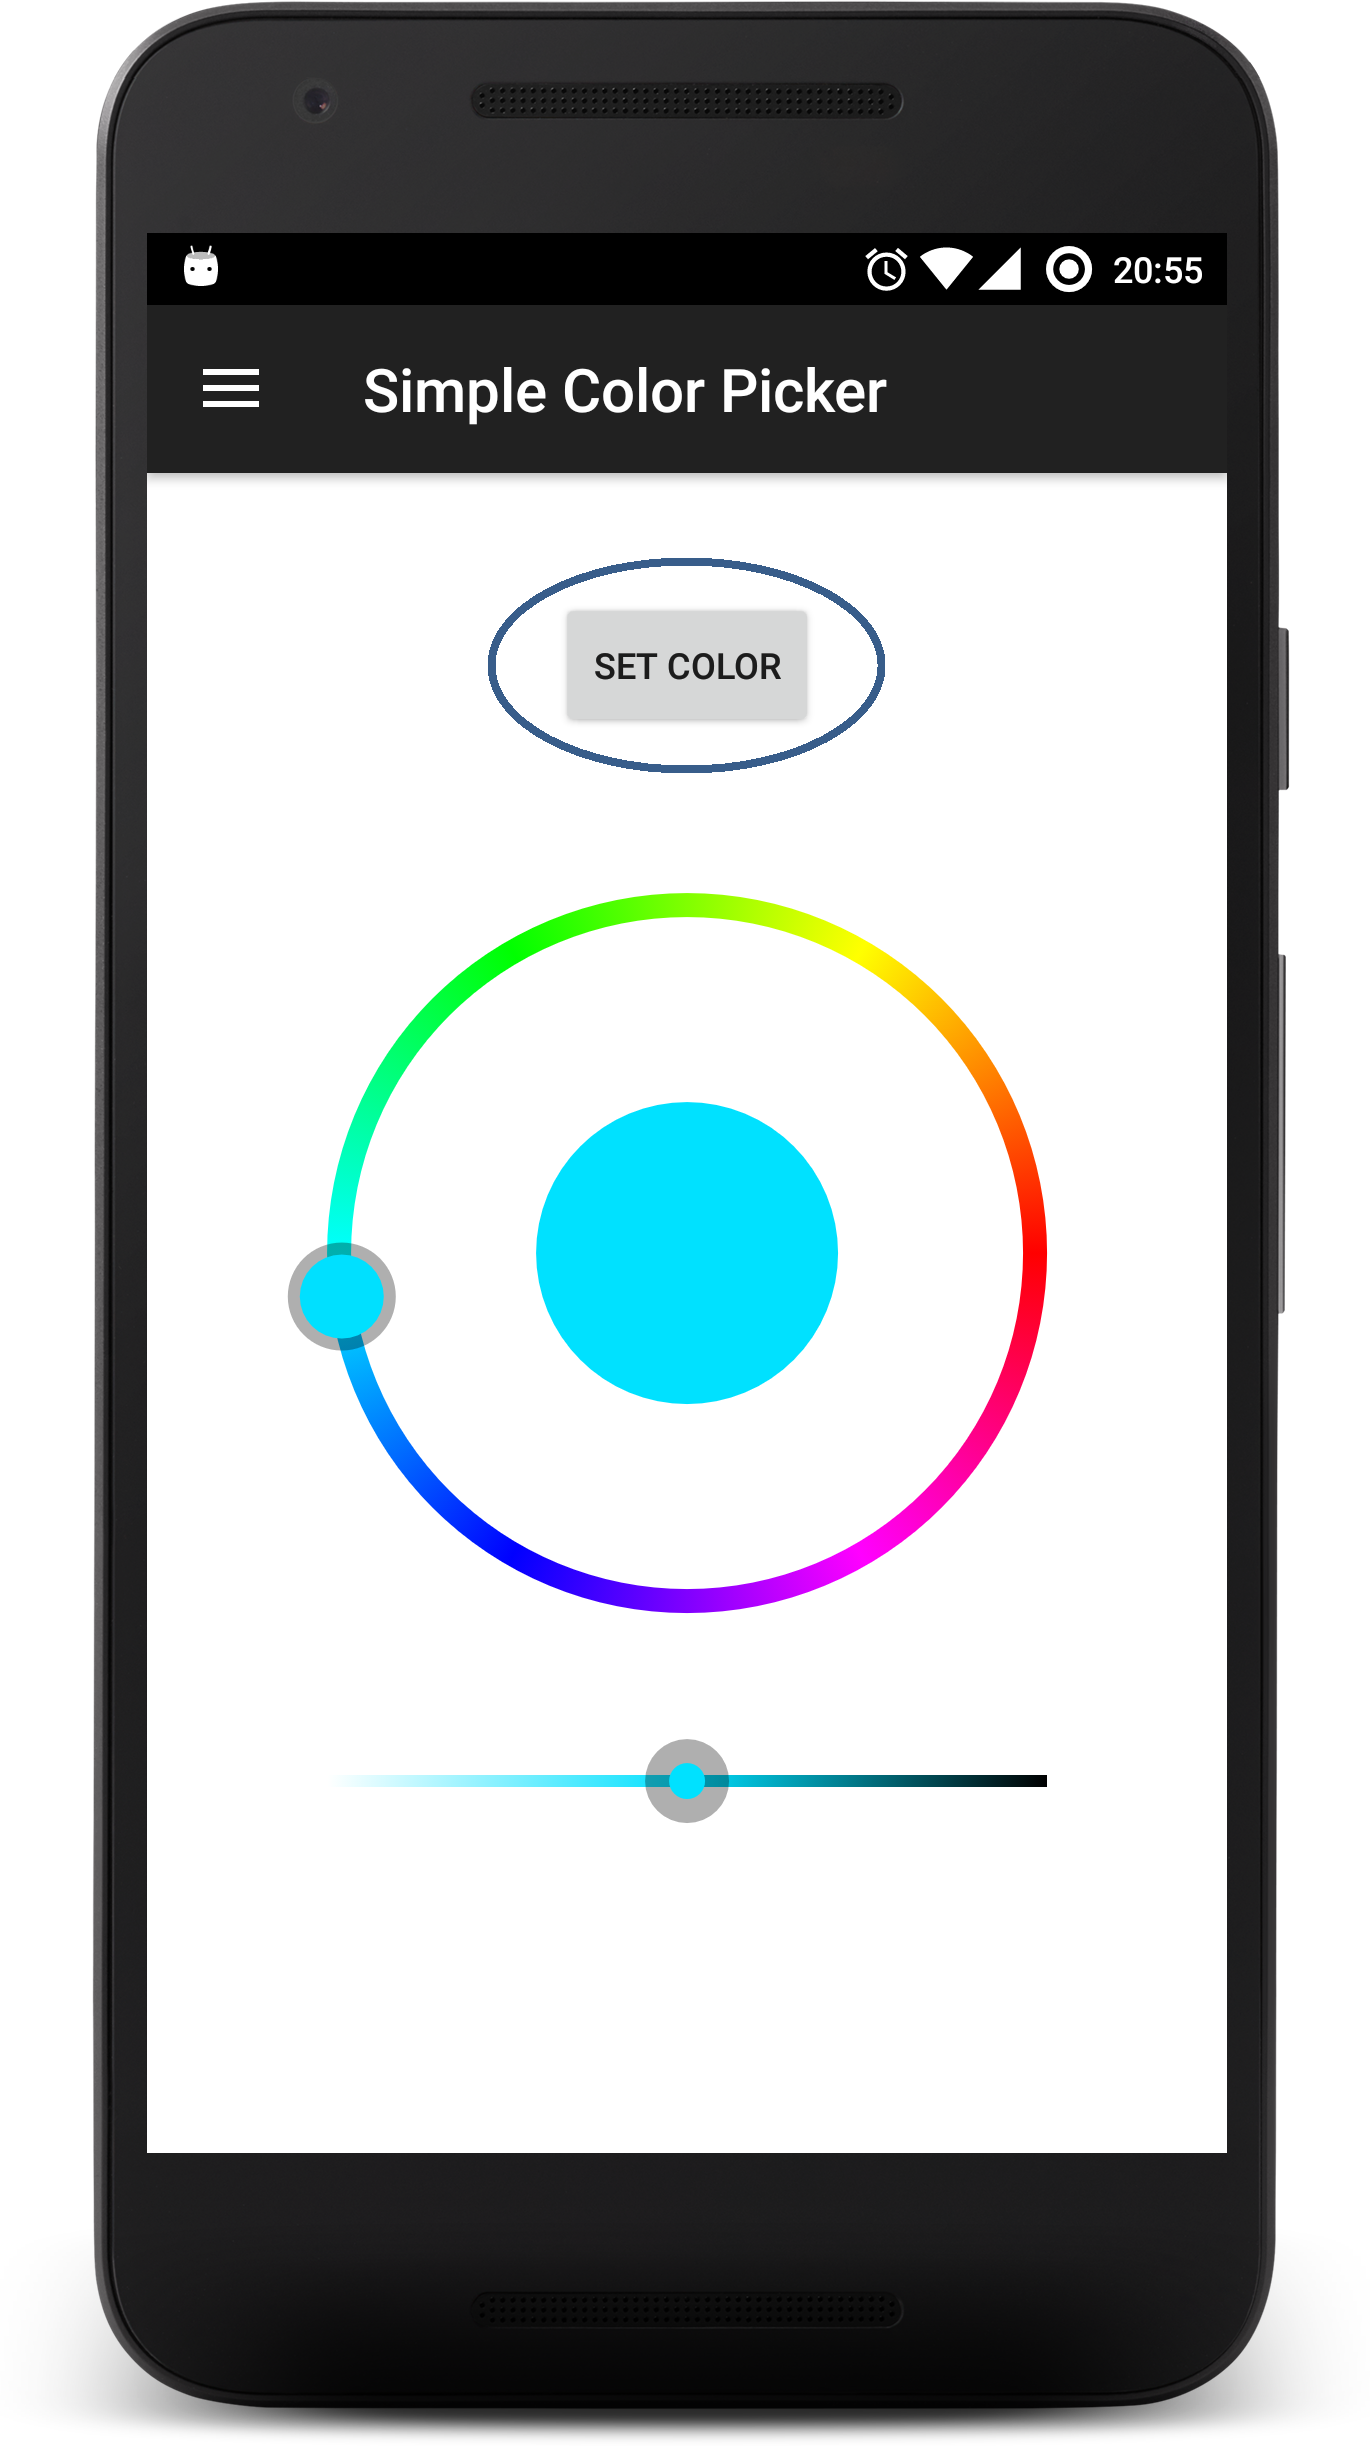
\includegraphics[width=5cm]{android_res/screen_pictures/s_cp_02.png}}{\caption{Szín beállítását a gombra koppintással végezhetjük el}\label{fig:s_cp_02}}
                \end{floatrow}
            \end{figure}\\
            
            A képernyőt személyre szabhatjuk a beállítások fülön lévő automata színválasztó funkció bekapcsolásával (Ábra ~\ref{fig:s_cp_03},~\ref{fig:s_cp_04}).
            
            \begin{figure}[h!]
                \begin{floatrow}
                    \ffigbox{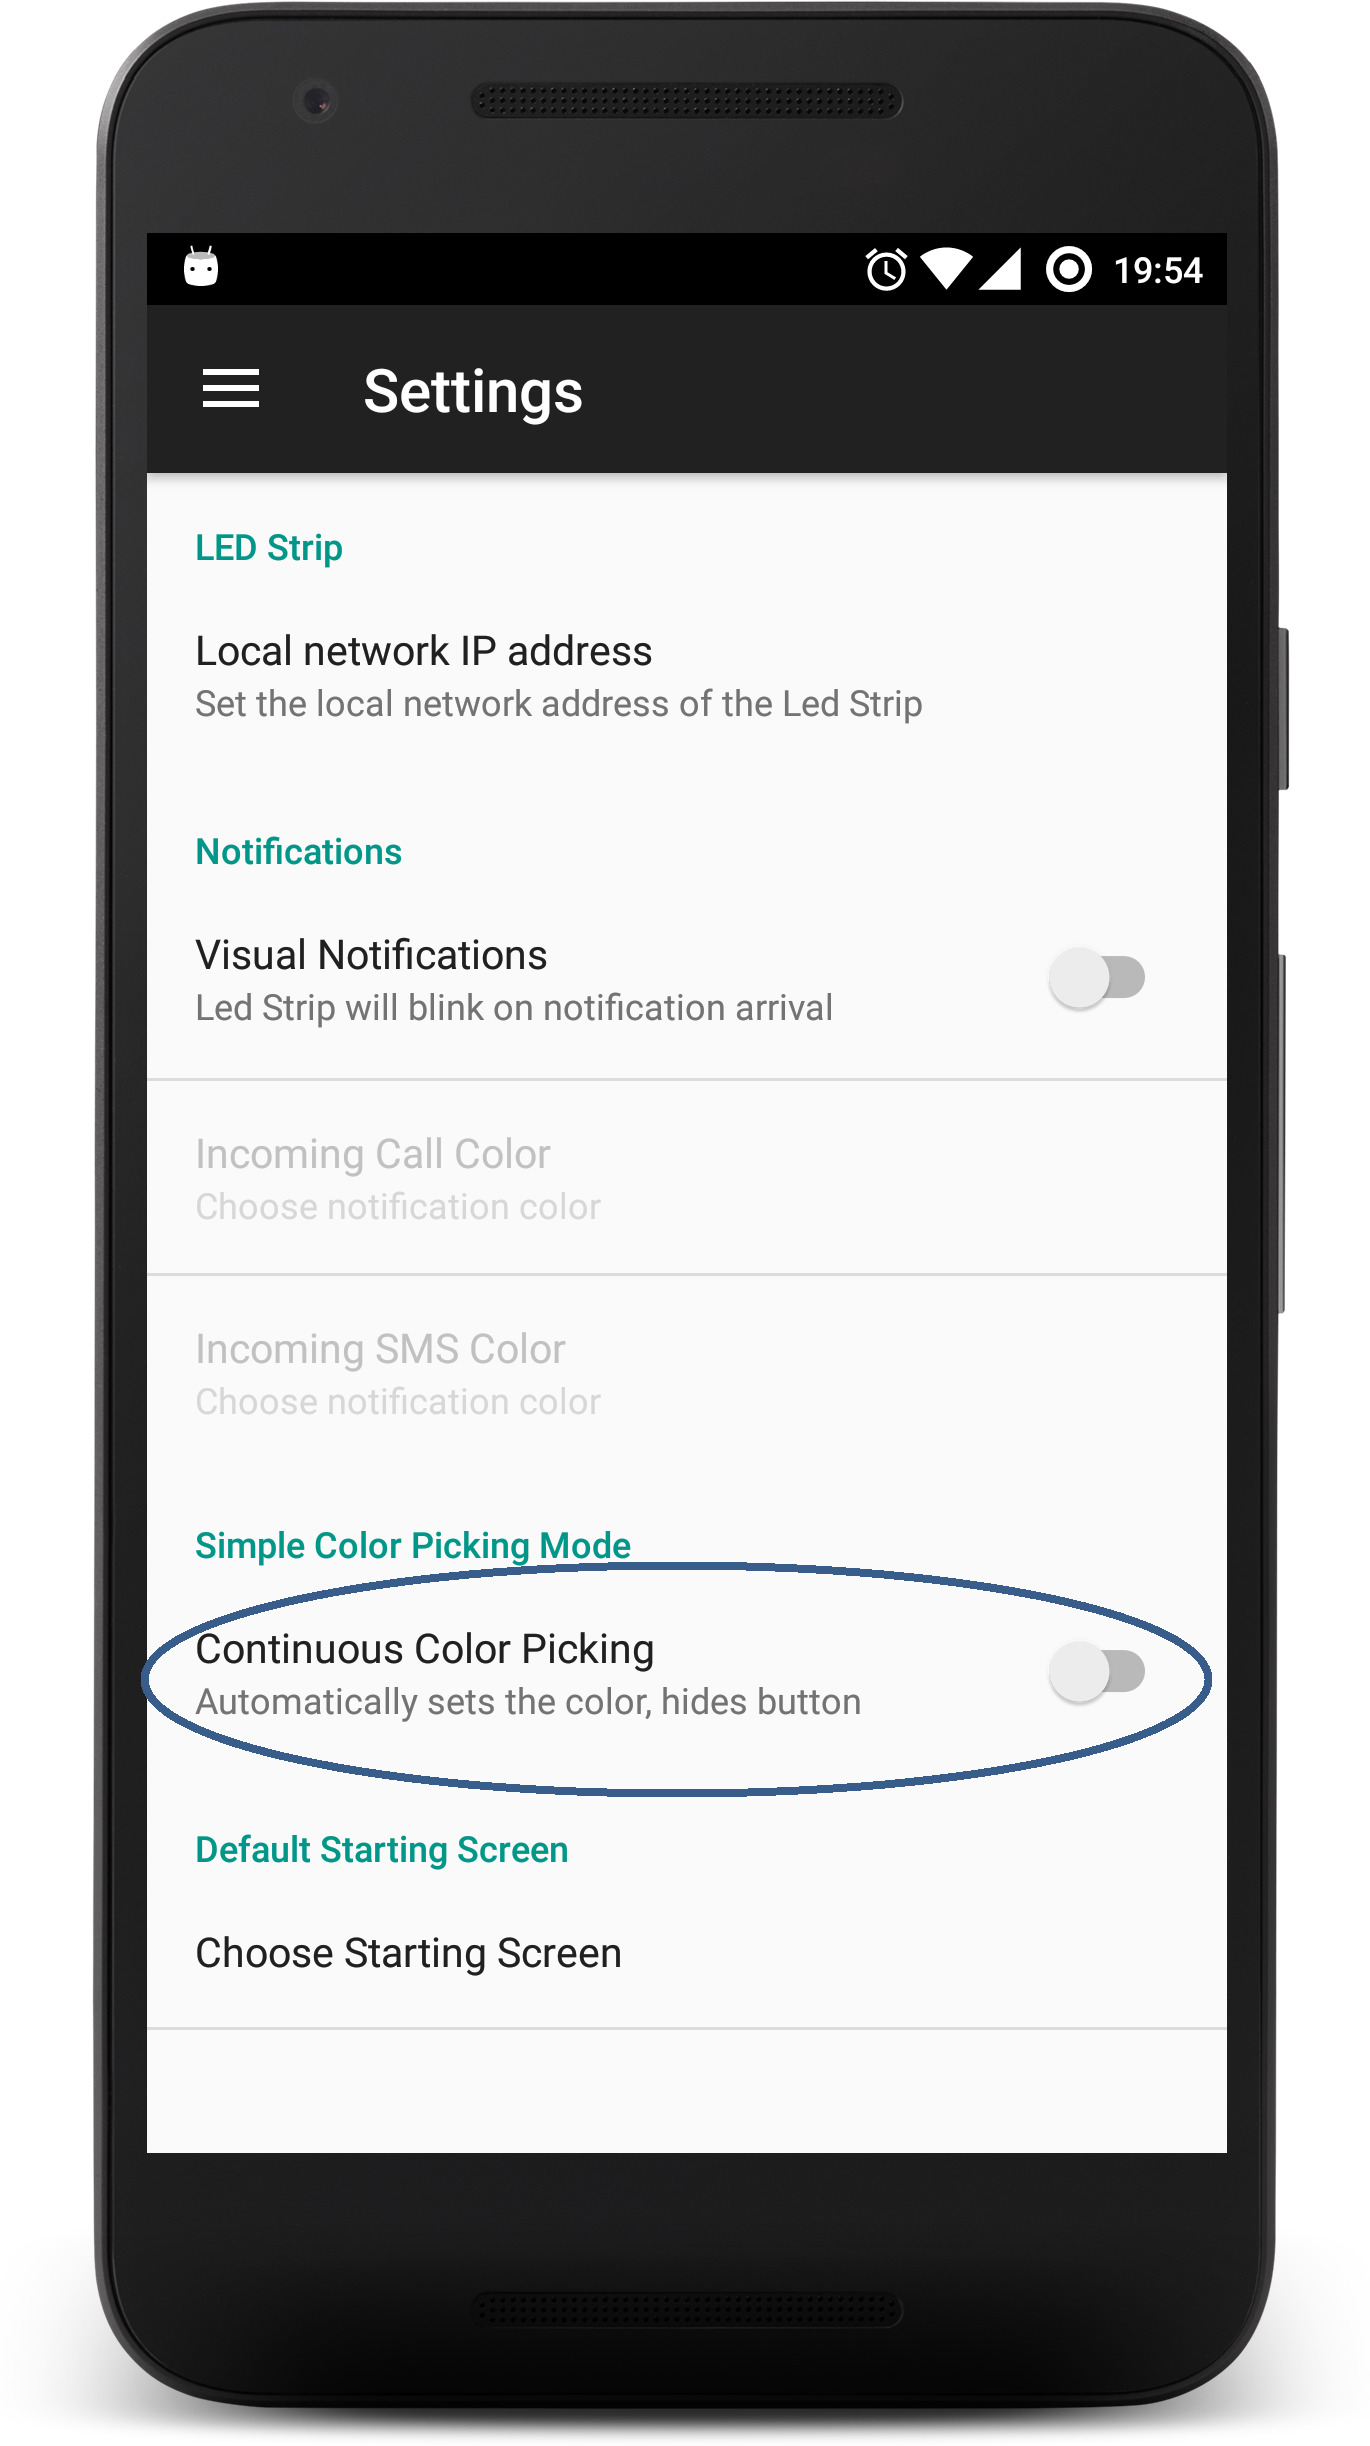
\includegraphics[width=5cm]{android_res/screen_pictures/s_cp_03.png}}{\caption{Automatikus színválasztás funkció bekapcsolása}\label{fig:s_cp_03}}
                    \ffigbox{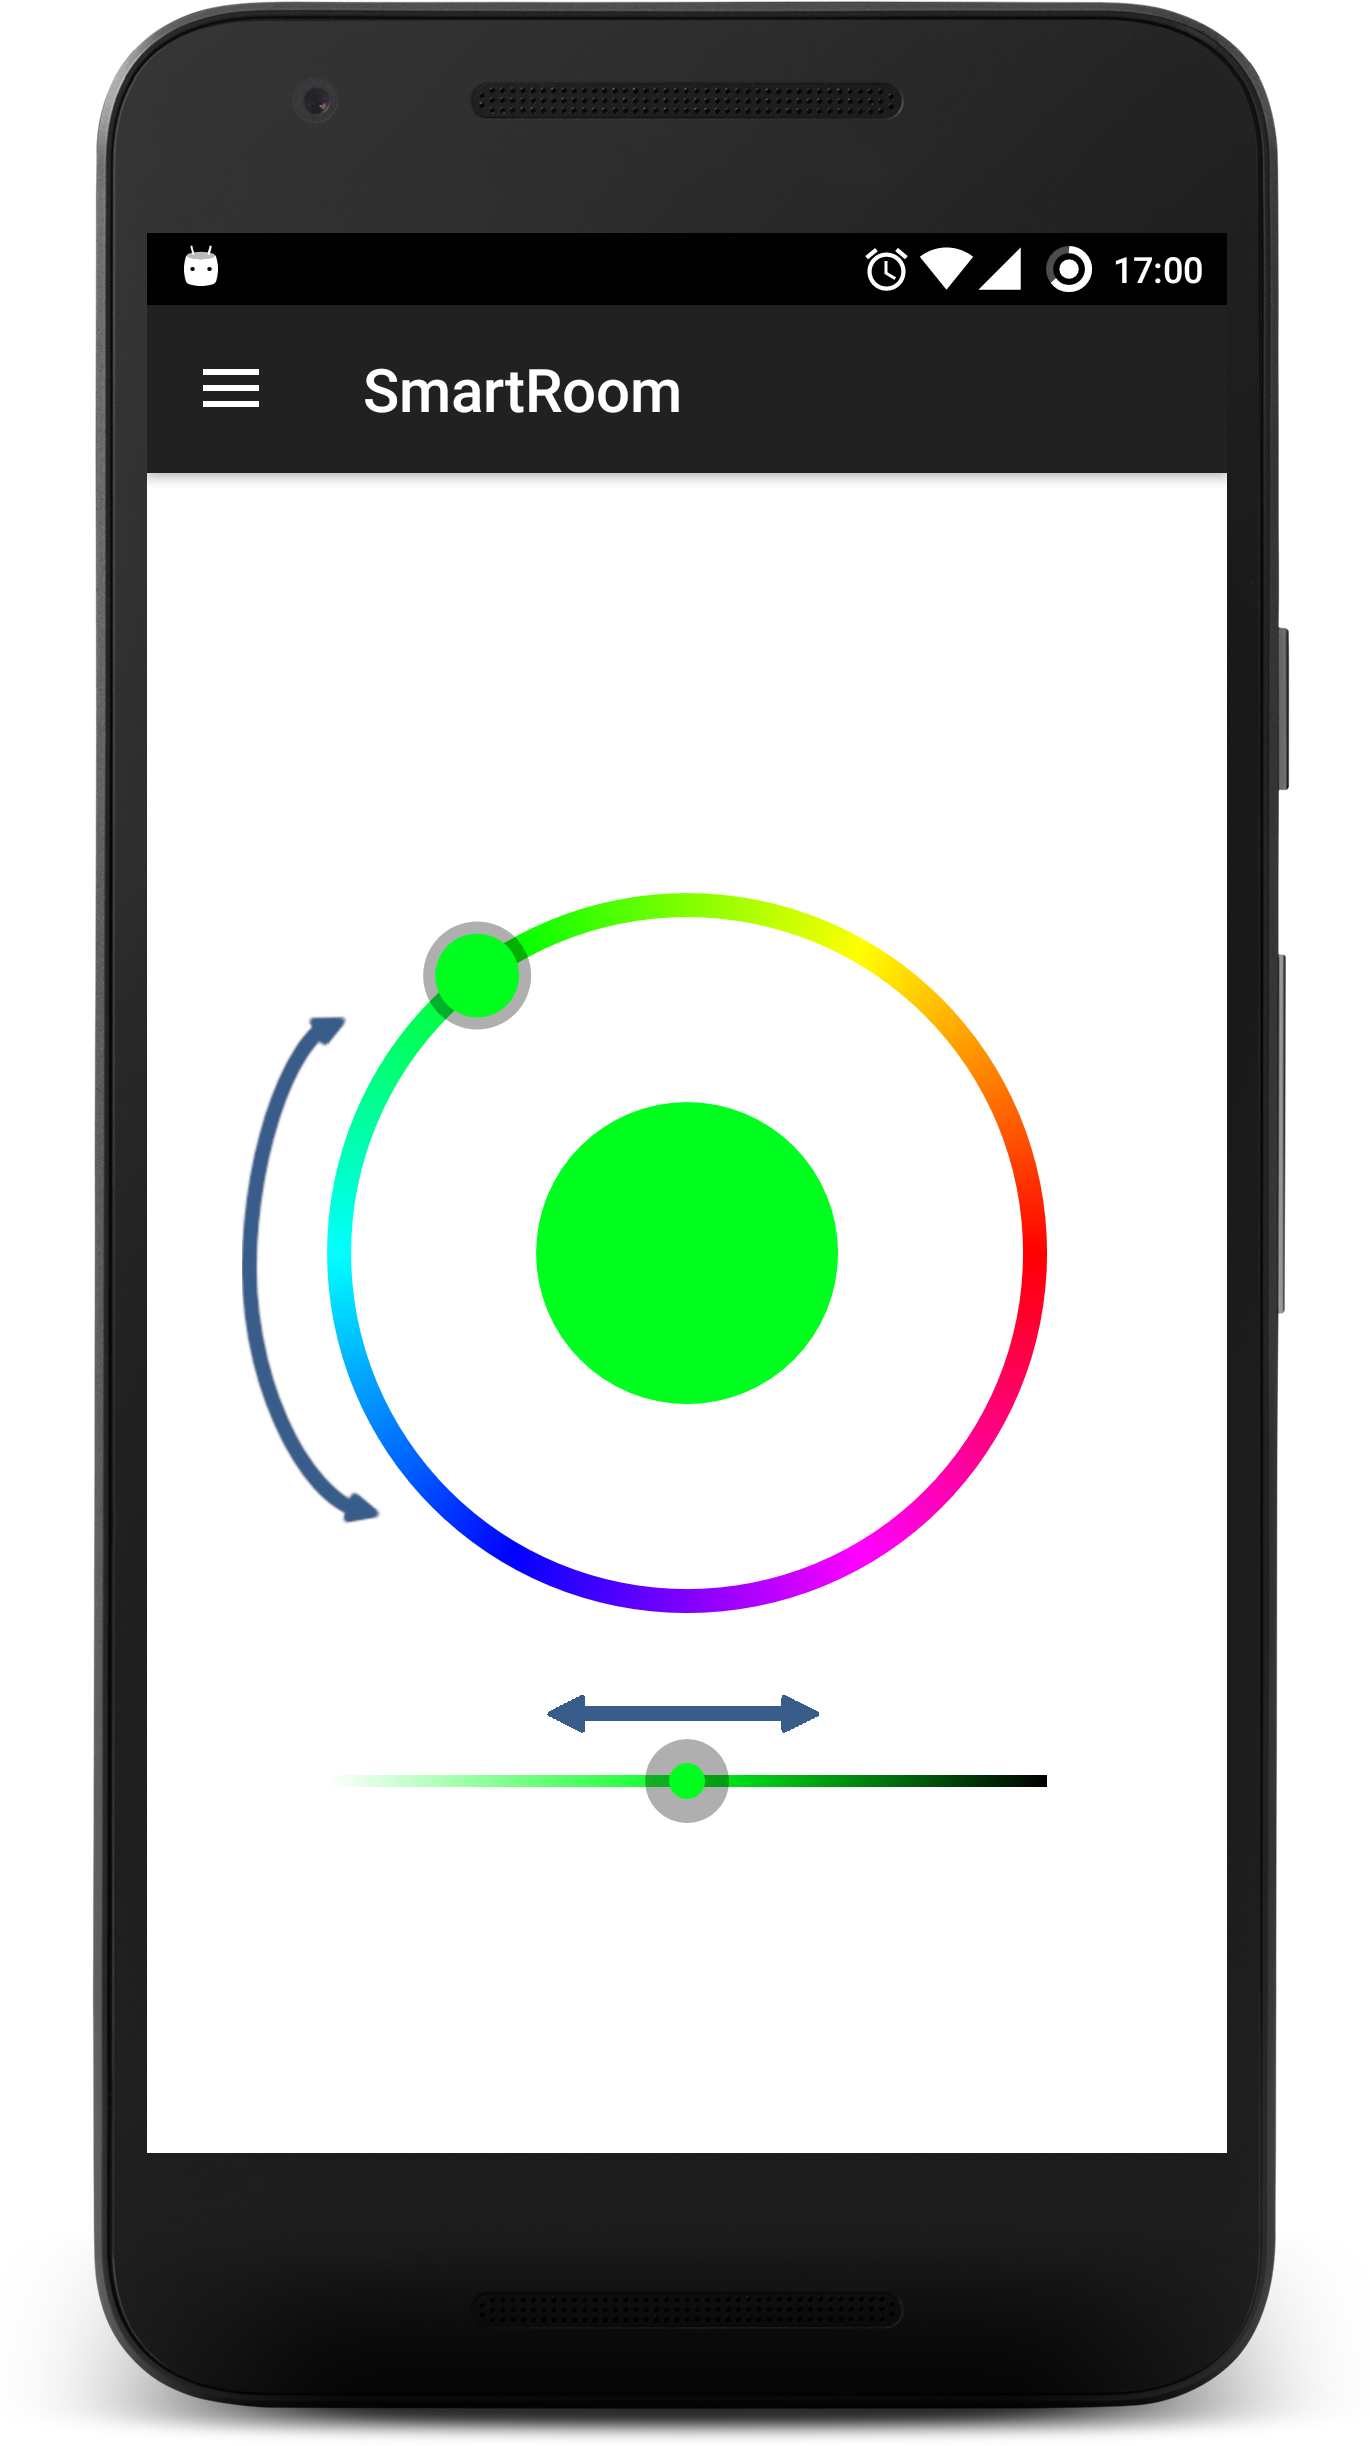
\includegraphics[width=5cm]{android_res/screen_pictures/s_cp_04.png}}{\caption{Ezek után a csúszkákat mozgatva automatikusan változtatja a színt}\label{fig:s_cp_04}}
                \end{floatrow}
            \end{figure}
            
\end{document}